This chapter presents a novel approach proposed by the author for clustering building plate areas characterized by similar thermal profiles, firstly described in \citeauthor{secchi_bagging_2013} (2013). In general, it can be applied to any functional data referenced by a lattice in $\mathbb{R}$, $\mathbb{R}^2$ or $\mathbb{R}^3$. The analysis of functional data allows us to gain a comprehensive and detailed understanding of the anomalies and the thermal history, which would enable us to discern if there are specific zones on the print plane behaving irregularly and to understand how hot spots might influence the mechanical properties of the printed part, given the fact that we have a functional knowledge of those phenomena. Section \ref{sec:fda} briefly introduces functional data analysis. Section \ref{sec:bvc} gives a detailed explanation of the Bagging Voronoi algorithm for geo-referenced functional data clustering, and Section \ref{sec:irradiance} presents a successful case study of the algorithm application.

% Functional Data Analysis >>>
\section{Functional Data Analysis}
\label{sec:fda}
This section discusses Functional Data Analysis (FDA) and Functional Principal Component Analysis (FPCA). It provides a brief overview to give readers the foundational knowledge needed to understand the algorithm described in Section \ref{sec:bvc}. This section is based mainly on \citeauthor{ramsay_functional_2006} (2006) and \citeauthor{ramsay_functional_2009} (2009).

Functional data are measurable observations of a given phenomenon that we can assume, with a fair degree of certainty, that a function can describe it. Indeed, although each observation is a single discrete value, these values reflect the smooth behavior of the generative function of those data. Fig. \ref{fig:bambine} shows the height data in \unit{\centi\metre} of 10 girls measured at 31 different temporal instants in the Berkeley Growth Study. We can see the smooth behavior typical of analytic functions, suggesting a "height" function, relating height to girls' age. Like all mathematical functions, the height function has interesting properties, including continuity and the possibility to compute function derivatives. Indeed, we can calculate the first derivative of the height function and interpret it as the growth velocity. Similarly, we can calculate the second derivative, the growth acceleration, as Fig. \ref{fig:accelerazione} shows.
\begin{figure}
    \centering
    \subfloat[\label{fig:bambine}]{
        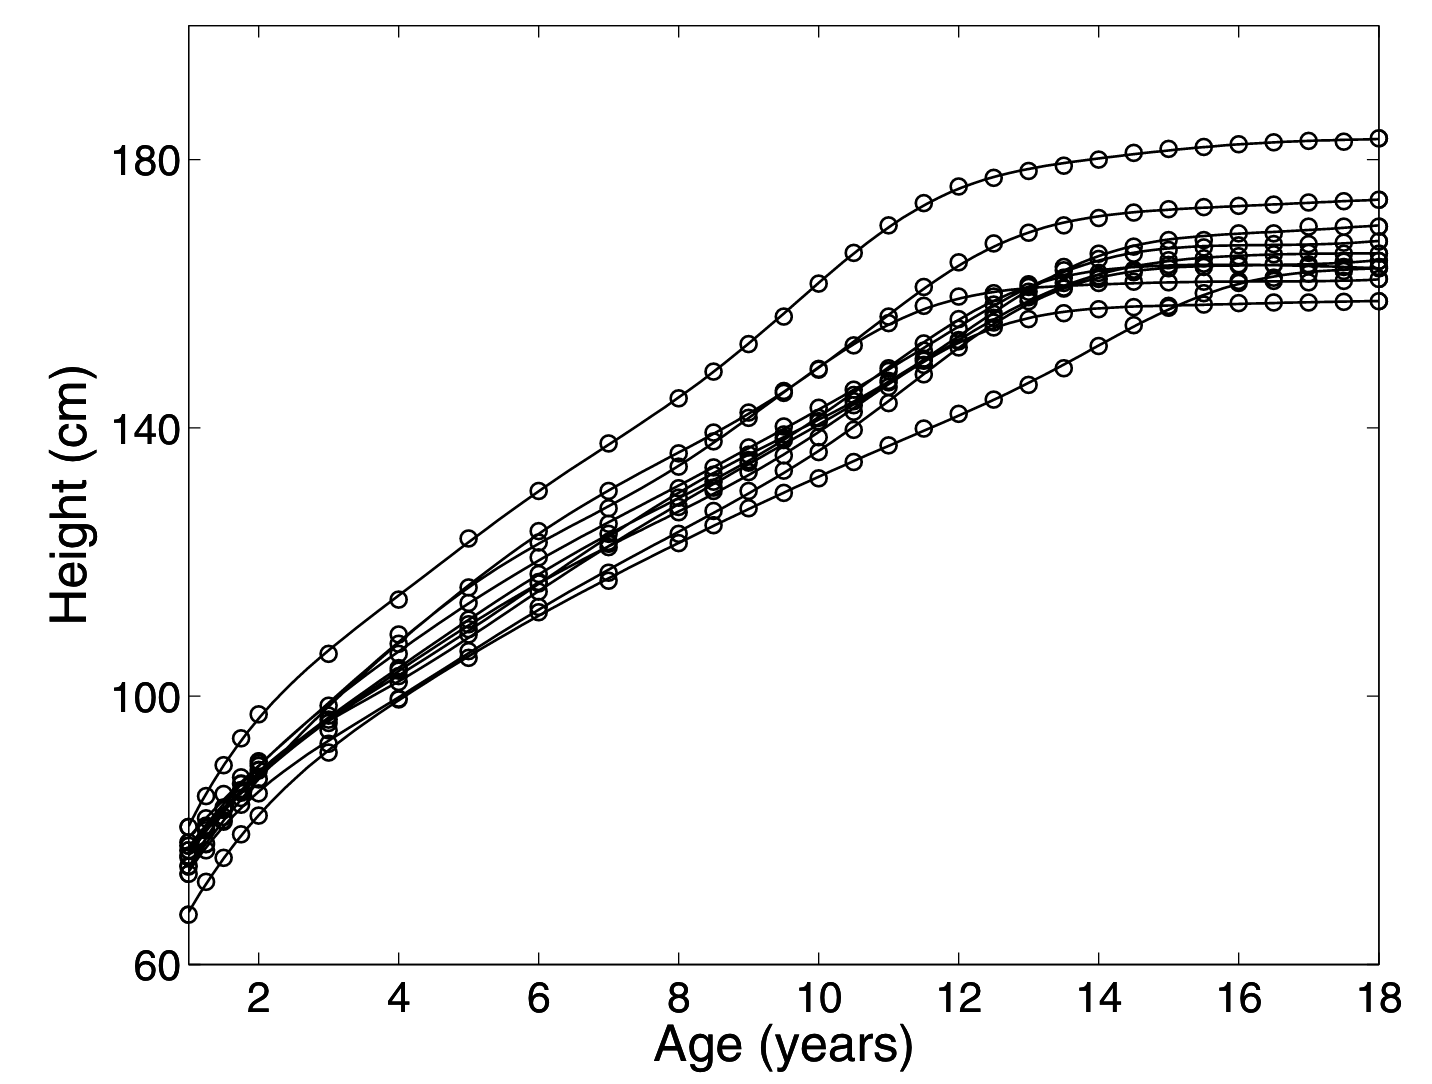
\includegraphics[scale=0.28]{Images/crescita.png}
    }
    \qquad
    \subfloat[\label{fig:accelerazione}]{
        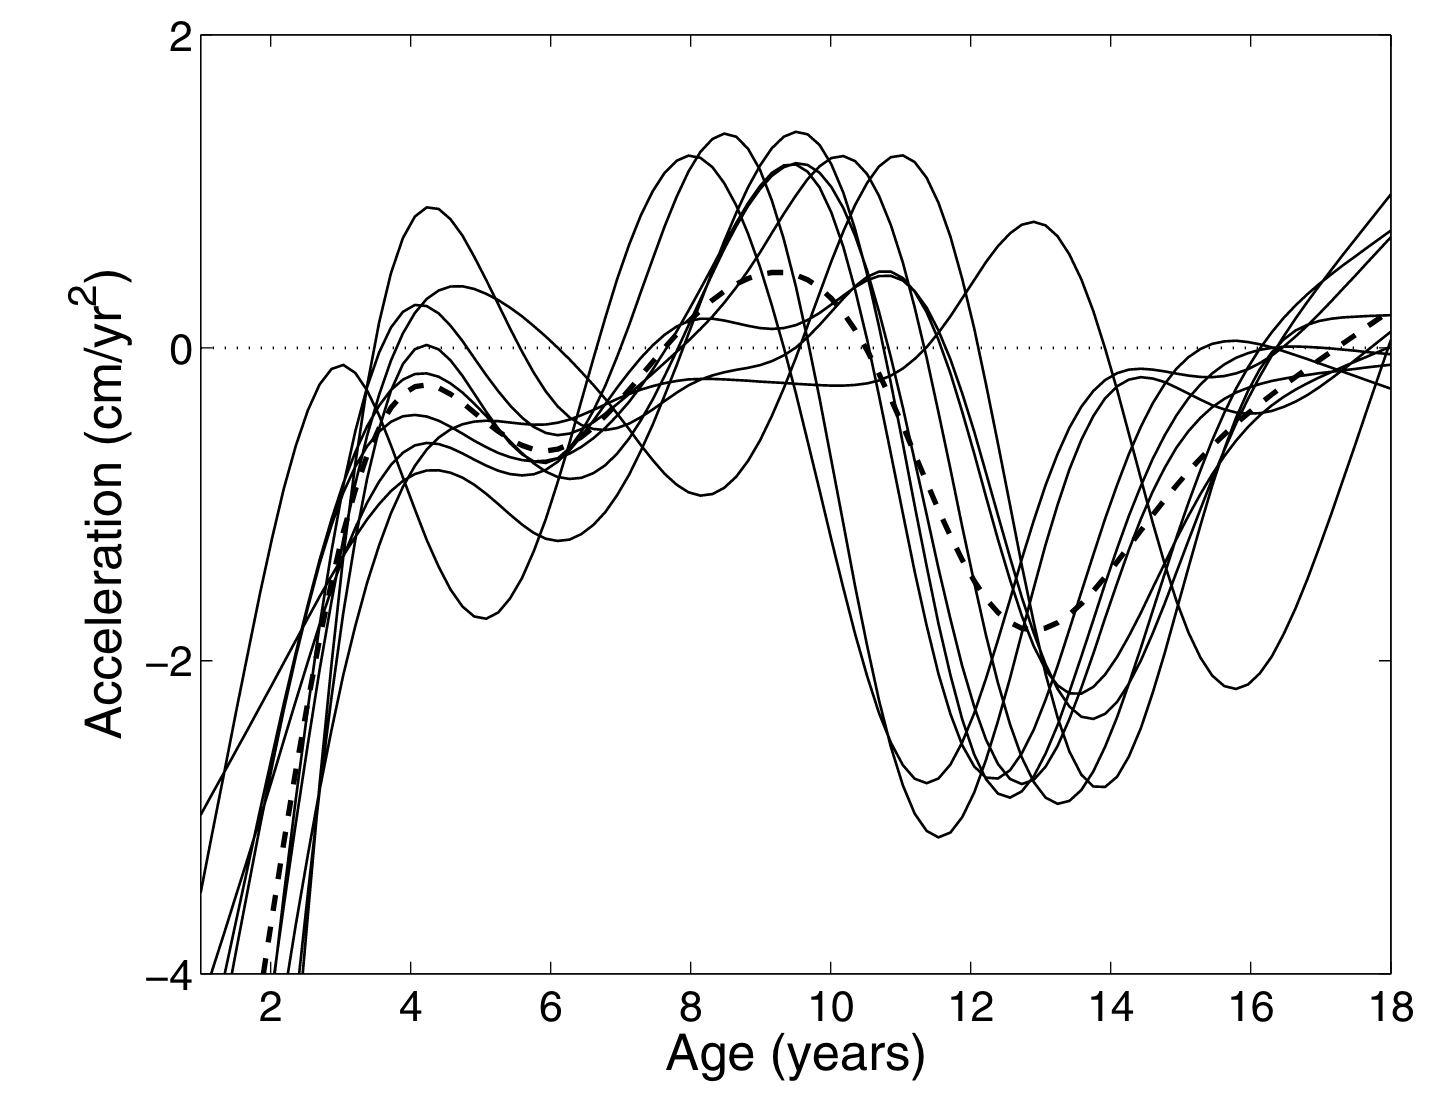
\includegraphics[scale=0.28]{Images/accelerazione.png}
    }
    \caption[Functional data]{The heights of 10 girls measured at 31 ages (a) and their estimated accelerations (b) \cite{ramsay_functional_2006}. The dotted line is the cross-sectional mean acceleration.}
    \label{fig:tuttoinsieme}
\end{figure}
Even if the height observations are taken nominally at the same age for each girl, it is not strictly needed. Indeed, the points at which the function is observed may change from one subject to another. It can be helpful in quality control that relies on sensors we discussed in Section \ref{sec:sensoriniiniini} to deal with missing values due, for example, to the obstruction of the off-axis sensor by the recoating blade. Furthermore, the signals transmitted by these sensors may be affected by disturbances that prevent the observed quantity from being correctly measured, causing discontinuities or missing values. It is also important to note that the FDA does not suffer from the problems of classical multivariate methods. It can also be used when the number of variables $p$ is larger than the available sample size $n$. In the case of Fig. \ref{fig:tuttoinsieme}, we have $p=31$ and $n=10$. In general, the goal of the FDA is to represent data as functions, to provide a representation that helps to analyze and highlight various characteristics of the collected data. This allows us to explain patterns of variation in the data and compare data containing different sets of observations of the same function or functions for a standard set of replicates. We can write each functional observation as the sum of a functional component and a random component that we will call noise. Formally, we can write every observed profile $y_j$ as 
\begin{equation}
    y_j = f(t_j) + \varepsilon_j \qquad \varepsilon_j\sim N(0, \sigma_j^2)
\end{equation}
We can approximate the unknown functional component as a linear combination of a functional basis. A basis function system is a set of known functions $\phi_k$ such that they are mathematically independent of each other and have the property that they can arbitrarily well approximate any function by taking a weighted sum (linear combination) of a sufficiently large number $K$ of these functions.
\begin{equation}
\label{eq:linear}
    \hat{f}(t)=\sum_{k=1}^K c_k \phi_k(t)
\end{equation}
Now, let $\mathbf{c}$ indicate the vector of length $K$ of the coefficients $c_k$ and $\bm{\phi}$ as the functional vector whose elements are the basis functions $\phi_k$, we can also express \ref{eq:linear} in matrix notation as
\begin{equation}
\label{eq:matrice}
    \hat{f}(t)=\mathbf{c}'\bm{\phi}=\bm{\phi}'\mathbf{c}
\end{equation}
When $K=n$, we have a limit case called exact representation or interpolation. It is a limit situation because we can choose the coefficients of the weighted sum such that $\hat{f}(t_j)=y_j$ for each $j$. Thus, $K$ controls the smoothness of the approximation $\hat{f}(t)$. We have to choose this parameter according to the used functional basis and the characteristics of the data. Another parameter to be selected is the type of functional basis itself. There are different functional bases, each with different characteristics, which ideally reflect the features of observed data. In a certain way, we can use the parameter $K$ to understand whether the used basis was more or less suitable: the smaller $K$ is, the better the base reflects the characteristics of the data. The type of basis selected is critical when one is interested in analyzing derivatives. Formally, when we are interested in
\begin{equation}
    \label{eq:derivative}
    D \hat{f}(t)=\sum_k^K \hat{c}_k D \phi_k(t)=\hat{\mathbf{c}}^{\prime} D \phi(t)
\end{equation}
where $D$ is the derivative operator defined as $Df(t)=\frac{d}{dt}f(t)$. This operator can also define further derivatives as powers of $D$.
\begin{equation}
    \label{eq:deroperator}
    D^2f(t)=\frac{d^2}{dt^2}f(t), \dots, D^kf(t)=\frac{d^k}{dt^k}f(t)
\end{equation}
The following are some of the most common functional bases used, highlighting their characteristics.
\paragraph{Polynomial basis.} The polynomial basis consists of monomials of different order.
\begin{equation}
    \label{eq:polinomial}
    \phi_k(t)=(t-\omega)^k \qquad k=0,\dots, K
\end{equation}
where $\omega$ is a shift parameter that is usually chosen to be in the center of the interval of approximation. The polynomial basis tends to fit the center of the data very well, but the tails tend to exhibit less ideal behavior. This is why they are never used for extrapolation or forecasting. However, the basis has a remarkable behavior: if $t_j$ are equally spaced, the basis can be fit with minimal computational effort. Moreover, derivatives are simple to compute and tend to be good estimators for actual derivatives, although they may present a wiggling effect when $K$ is excessively large. 
\paragraph{Exponential and power basis.} The exponential base consists of a series of exponential functions 
\begin{equation}
    \label{eq:exponential}
    \phi_k(t)=\exp (\lambda_kt) \qquad k=1,\dots, K
\end{equation}
where the rate parameters $\lambda_k$ are all distinct and often $\lambda_1=0$. This basis is particularly useful as linear differential equations with constant coefficients have expansions in terms of an exponential basis as solutions. While power basis
\begin{equation}
    \label{eq:power}
    \phi_k(t)=t^{\lambda_k} \qquad k=1,\dots, K
\end{equation}
is less useful, but can be helpful when $t$ is strictly positive.
\paragraph{Fourier basis.} One of the most famous and widely used bases is the Fourier basis, mainly because it can capture the periodic behavior of data and is very useful for stable functions when curvatures tend to have the same order in all the data. However, the Fourier basis is unsuitable for data known or suspected to reflect some discontinuities. Fourier basis is defined as:
\begin{equation}
    \label{eq:fourier}
    \phi_k(t)=\left\{ \begin{array}{ll}
         \phi_k(t)=1 & \text{for} \quad k = 0 \\
         \phi_{2k-1}(t)= \sin(k\omega t) & \text{for} \quad k = 1, \dots, K \\
         \phi_{2k}(t)= \cos(k\omega t) & \text{for} \quad k = 1, \dots, K
    \end{array}\right.
\end{equation}
The period of the basis is determined as $\mathcal{T}=\frac{2\pi}{\omega}$. The algorithm used to calculate the coefficients of this basis, the Fast Fourier transform, makes it possible to find the coefficients extremely efficiently when $n$ is a power of 2 and the observations are equally spaced.
\paragraph{B-splines basis.} The B-splines base is a splines base. Splines are bases defined by a number $L$ of knots and an order $m$. Knots are values $\tau_l$ for $l=1,\dots,L-1$ that divide the interval on which a function has to be estimated into $L$ sub-intervals. On each sub-interval, the spline is a polynomial function of a specific order $m$ which is the degree of the polynomial itself. Polynomials defined on adjacent intervals join smoothly at knot values, such that the function at that point is constrained to the value of the knot itself. By increasing the number of knots, the fit of the estimated function to the observed data can be improved up to the extreme situation where the knot numbers have the same value as the observed data. Thus, the number of nodes will affect the goodness of fit to the observed data. In a certain way, the parameter $L$ regulates the flexibility of our fit. This is why having more nodes is a good practice for regions with complex variations. Thus, to summarise what has been said so far, a spline is defined by the order of the polynomials and the sequence of nodes. B-splines are a particular spline basis developed by de Boor in 2001. 
\begin{figure}
\centering
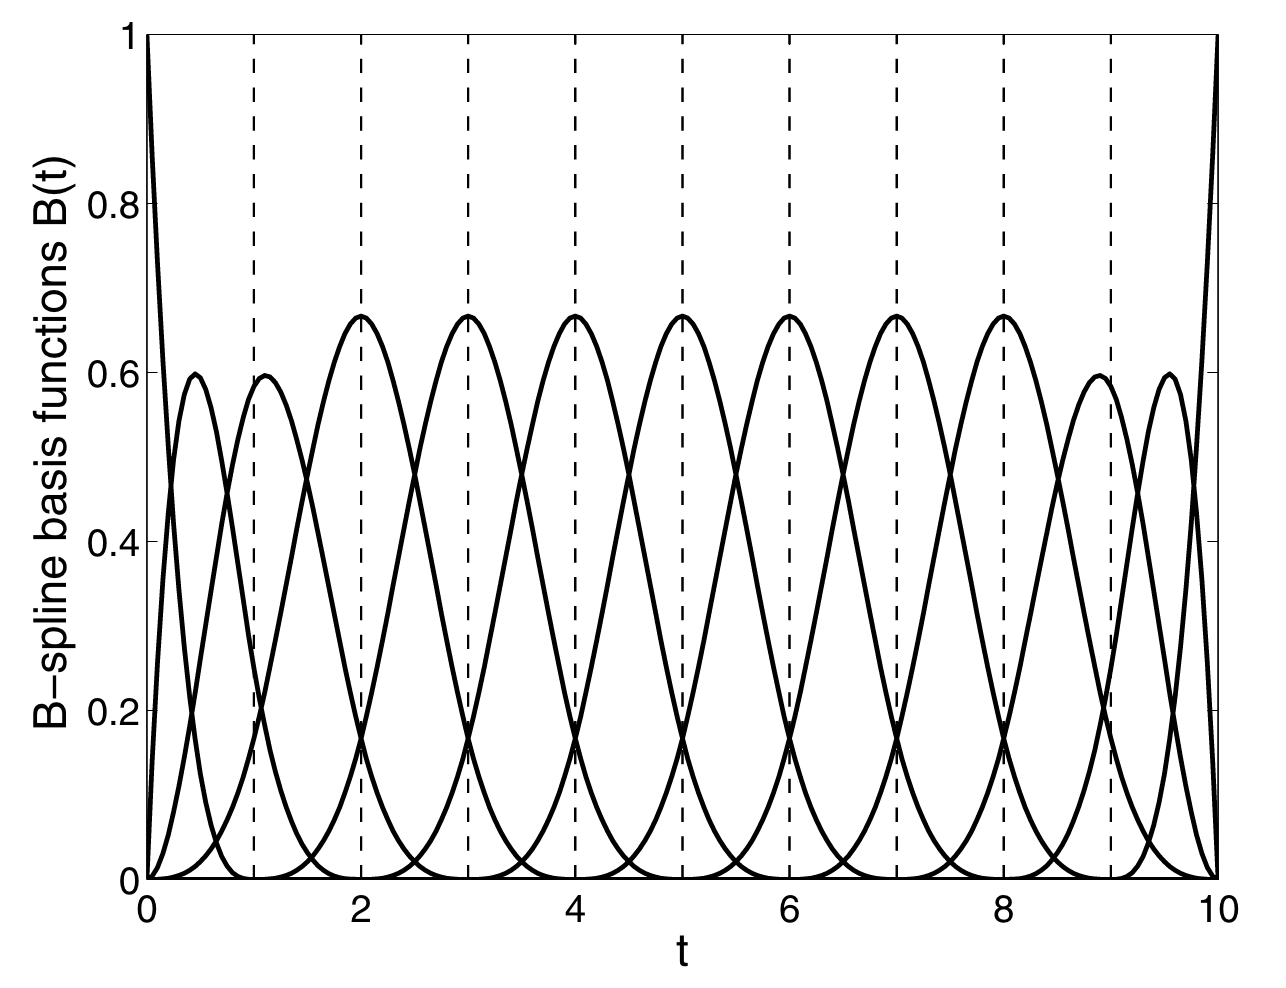
\includegraphics[width=0.4\textwidth]{Images/bspline.png}
\caption[Bsplines fitting.]{The thirteen basis functions defining an order four spline with nine interior knots, shown as vertical dashed lines \cite{ramsay_functional_2006}.}
\label{fig:bspline_13}
\end{figure}

\begin{figure}
\centering
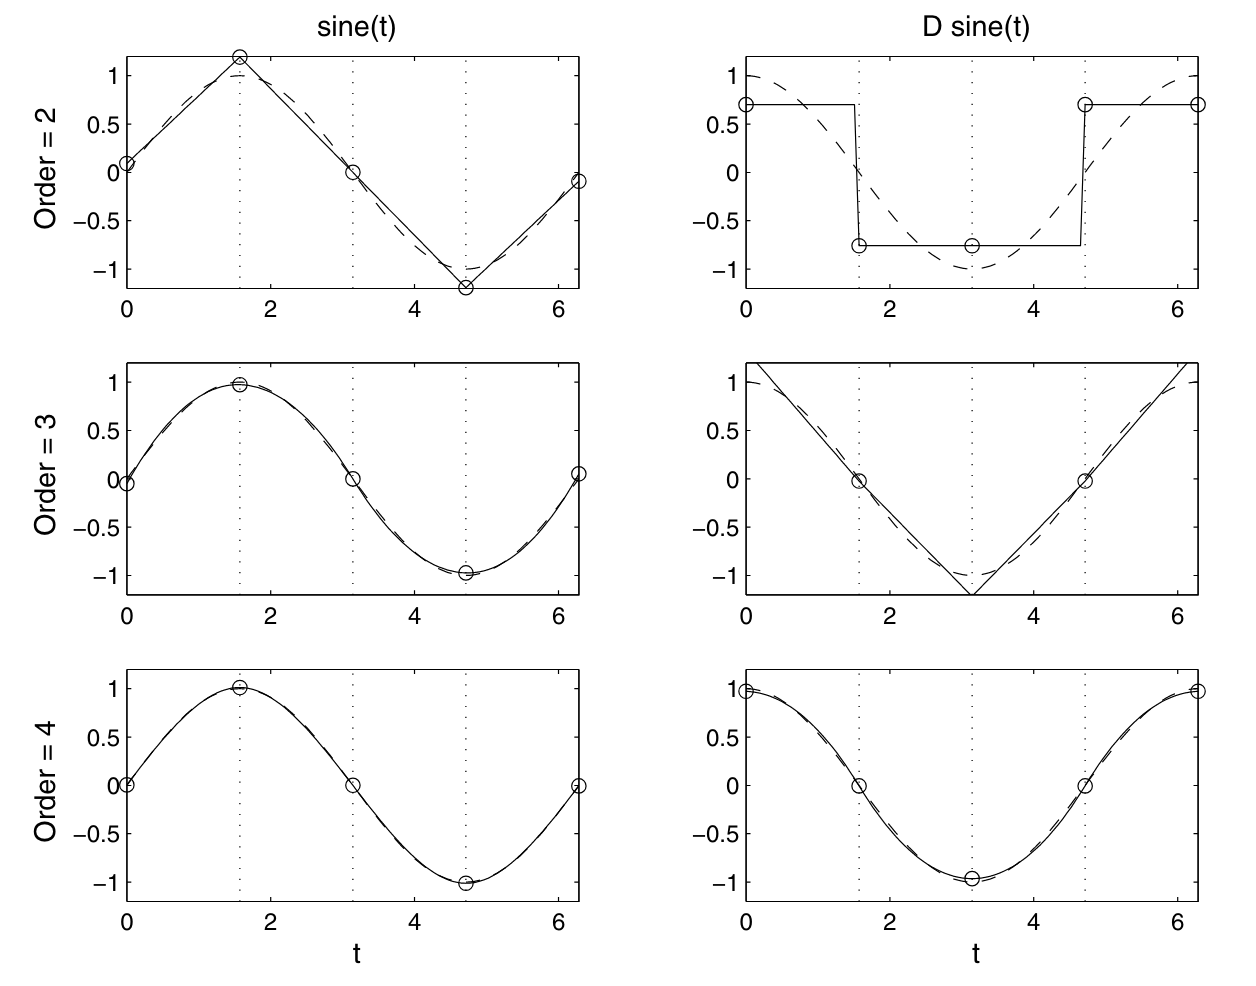
\includegraphics[width=0.7\textwidth]{Images/bsplines.png}
\caption[Bsplines fitting.]{In the left panels the solid line indicates spline function of a particular order that fits the sine function shown as a dashed line. In the right panels the corresponding fits to its derivative, a cosine function, are shown. The vertical dotted lines are the interior breakpoints or knots defining the spline fits \cite{ramsay_functional_2006}.}
\label{fig:bsplines}
\end{figure}
From Fig. \ref{fig:bspline_13}, we can see that the three functions on the left and the last three on the right are different from the other. When transitioning from the left edge toward the center, the spans in which these functions remain positive expand from one to four. Yet, they consistently have the same smooth transition that's twice-differentiable. On the other hand, if we move from the center to the left or right, functions have different levels of smoothness: the far-left spline is discontinuous, the following one is only continuous, and the last is differentiable once. It makes perfect sense that we experience a loss in differentiability at the edges, given that we typically lack knowledge about the behavior of the function we're approximating outside the interval.
\paragraph{Wavelets basis.} We can construct a basis for all functions on $\left(- \infty, \infty \right)$ that are square integrable by choosing a suitable mother wavelet function $\psi$ and then considering all dilations and translations of the form
\begin{equation}
    \label{eq:wavelet}
    \psi_{j k}(t)=2^{j / 2} \psi\left(2^j t-k\right)
\end{equation}
for integers $j$ and $k$. The wavelet expansion of a function $f$ gives a multiresolution analysis in the sense that the coefficient of $\psi_{jk}$ yields information about $f$ near position $2^{-j}k$ on scale $2^{-j}$, i.e., at frequencies near $c2^j$ for some constant $c$. Wavelets are suitable for modeling sharp local features, even discontinuity, localized in space and frequency, which can be computed efficiently. Multidimensional wavelets provide coherent estimates of ECG traces, where the different projections of the heart dynamics are consistent.
\paragraph{Fit model to data.} There are different ways to fit a model to observed data. When we have to estimate a model, we want the model to fit our data somehow. To quantify how well it fits, we can define the concept of sum of squared errors defined as
\begin{equation}
    \label{eq:sse}
    \operatorname{SSE}(\mathbf{y} \mid \mathbf{c})=\sum_{j=1}^n\left[y_j-\sum_k^K c_k \phi_k\left(t_j\right)\right]^2
\end{equation}
or equivalently, we can re-write it in matrix form as
\begin{equation}
    \label{eq:ssematrix}
    \operatorname{SSE}(\bm{y} \mid \mathbf{c})=(\mathbf{y}-\bm{\Phi} \mathbf{c})^{\prime}(\mathbf{y}-\bm{\Phi} \mathbf{c})
\end{equation}
where $\bm{\Phi}$ is the $n \times K$ matrix containing the values $\phi_k(t_j)$. By deriving equation \ref{eq:ssematrix} with respect to $c$, we obtain equation
\begin{equation}
 \label{eq:c}
    2 \bm{\Phi} \bm{\Phi}^{\prime} \mathbf{c}-2 \bm{\Phi}^{\prime} \mathbf{y}=0
\end{equation}
and solving for $\mathbf{c}$, this provides the estimate $\hat{\mathbf{c}}$ that minimizes the least squares solution
\begin{equation}
    \label{eq:cestimated}
    \hat{\mathbf{c}}=\left(\bm{\Phi}^{\prime} \bm{\Phi}\right)^{-1} \bm{\Phi}^{\prime} \mathbf{y}
\end{equation}
The vectore $\hat{\mathbf{y}}$ of fitted values is
\begin{equation}
    \hat{\mathbf{y}}=\bm{\Phi} \hat{\hat{\mathbf{c}}}=\bm{\Phi}\left(\bm{\Phi}^{\prime} \bm{\Phi}\right)^{-1} \bm{\Phi}^{\prime} \mathbf{y}
\end{equation}
If we want to fit a model on data with a non-stationary and/or auto-correlated stochastic component, however, we must use weighted least squares fits. In this case, equation \ref{eq:ssematrix} becomes

\begin{equation}
    \label{eq:wls}
    \operatorname{SSE}(\mathbf{y} \mid \mathbf{c})=(\mathbf{y}-\bm{\Phi} \mathbf{c})^{\prime} \mathbf{W}(\mathbf{y}-\bm{\Phi} \mathbf{c})
\end{equation}
where the matrix $\mathbf{W}$ is a symmetric positive definite matrix that allows for unequal weightin of squares and products of residuals. The matrix $\mathbf{W}$ is defined as
\begin{equation}
    \mathbf{W}=\bm{\Sigma}_e^{-1}
\end{equation}
where $\bm{\Sigma}_e^{-1}$ is the variance-covariance matrix for the noise. AS before, if we derive \ref{eq:wls} with respect to $\mathbf{c}$ and by solving the equation, we get the weighted least squares estimate $\hat{\mathbf{c}}$ of the coefficient vector $\mathbf{c}$ defined as
\begin{equation}
    \hat{\mathbf{c}}=\left(\bm{\Phi}^{\prime} \mathbf{W} \bm{\Phi}\right)^{-1} \bm{\Phi}^{\prime} \mathbf{W} \mathbf{y}
\end{equation}
Finally, in the case of a splines basis, we can smooth the model to the data by introducing a roughness penalty. We have already encountered the derivative operator in \ref{eq:deroperator}. The first two derivative operators are particularly relevant because  $Df(t)$ is the local slope of $f(t)$ and $D^2f(t)$ is its curvature. We can therefore define the roughness of the $m$-th derivative as
\begin{equation}
    \label{eq:roughness}
    \begin{aligned}
\operatorname{PEN}_m(x) & =\int\left[D^m x(s)\right]^2 d s \\
& =\int\left[D^m \mathbf{c}^{\prime} \boldsymbol{\phi}(s)\right]^2 d s \\
& =\int \mathbf{c}^{\prime} D^m \boldsymbol{\phi}(s) D^m \boldsymbol{\phi}^{\prime}(s) \mathbf{c} d s \\
& =\mathbf{c}^{\prime}\left[\int D^m \boldsymbol{\phi}(s) D^m \boldsymbol{\phi}^{\prime}(s) d s\right] \mathbf{c} \\
& =\mathbf{c}^{\prime} \mathbf{R} c
\end{aligned}
\end{equation}
We can then find the right trade-off between the fitting of the data and the smoothness of fitted curve by minimising the penalised sum of squared errors
\begin{equation}
    \label{eq:pensse}
    \operatorname{PENSSE}_\lambda(f)=[\mathbf{y}-f(\mathbf{t})]^T[\mathbf{y}-f(\mathbf{t})]+\lambda \operatorname{PEN}_2[f]
\end{equation}
where $\lambda$ is a smoothing arameter measuring the compromise between fit and smoothness. As $\lambda$ increases, roughness is increasingly penalized, and $\hat{f}(t)$ will become linear. As it decreases, the penalty is reduced, allowing $\hat{f}(t)$ to fit the data better. In Fig. \ref{fig:lambda}, we can see the different fit of yearly precipitations data of Vancouver obtained by using different values of $\lambda$.
\begin{figure}
    \centering
    \subfloat[\label{fig:-1}]{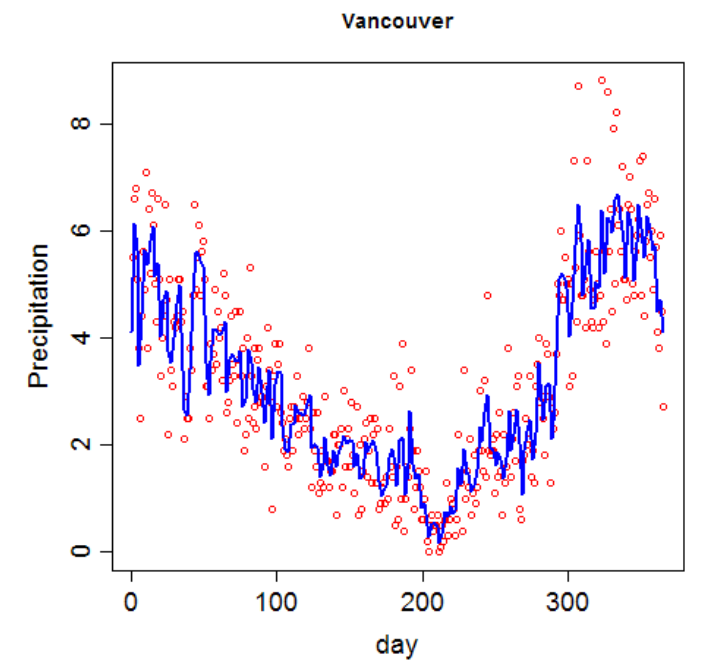
\includegraphics[width = 0.3\textwidth]{Images/-1.png}}
    \subfloat[\label{fig:7}]{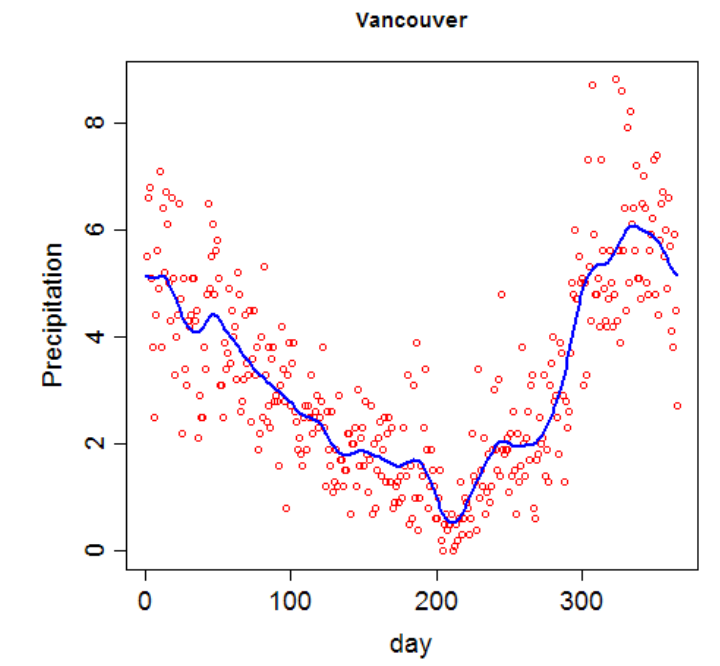
\includegraphics[width = 0.3\textwidth]{Images/7.png}}
    \subfloat[\label{fig:15}]{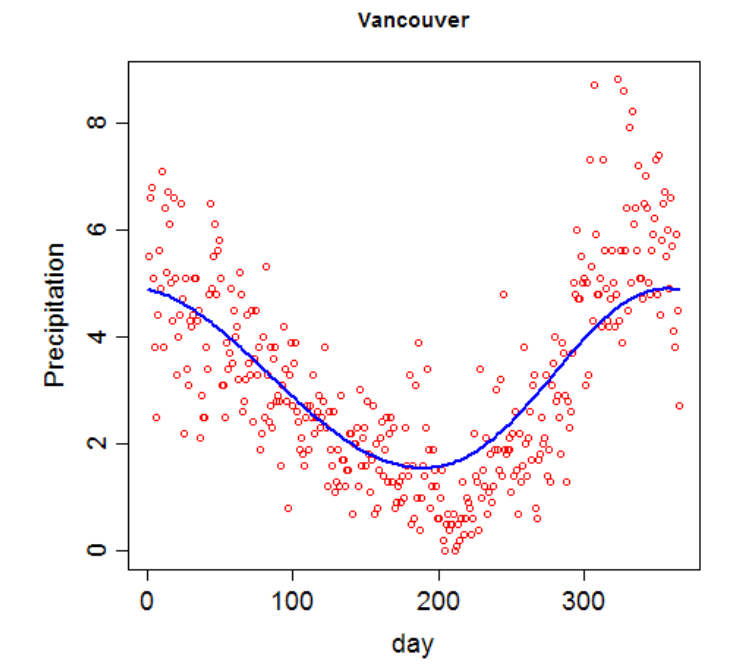
\includegraphics[width = 0.3\textwidth]{Images/15.png}}
    \caption[PENSSE with different $\lambda$]{PENSSE on Vancouver precipitations data with $\lambda=-1$ (a), $\lambda=7$ (b) and $\lambda=15$ (c) \cite{ramsay_functional_2009}.}
    \label{fig:lambda}
\end{figure}
Finally, the estimated coefficient vector $\hat{\mathbf{c}}$ will be 
\begin{equation}
    \hat{\mathbf{c}}=\left(\boldsymbol{\Phi}^{\prime} \mathbf{W} \boldsymbol{\Phi}+\lambda \mathbf{R}\right)^{-1} \boldsymbol{\Phi}^{\prime} \mathbf{W} \mathbf{y}
\end{equation}
and thus the data-fitting vector $\mathbf{\hat{y}}$ is
\begin{equation}
    \label{eq:unbelcasino}
    \hat{\mathbf{y}}=\boldsymbol{\Phi}\left(\boldsymbol{\Phi}^{\prime} \mathbf{W} \boldsymbol{\Phi}+\lambda \mathbf{R}\right)^{-1} \boldsymbol{\Phi}^{\prime} \mathbf{W} \mathbf{y}=\mathbf{S}_{\phi, \lambda} \mathbf{y}
\end{equation}
\paragraph{Choose the number $K$ of basis functions.} As we have seen in previous paragraphs, increasing the number of basis functions $K$ can increase the goodness of fit. Indeed, the larger $K$, the better the fit to the data. However, by increasing $K$ disproportionately, our model would also capture the stochastic component of the noise. On the other hand, by decreasing $K$ too much, we may risk missing some data features. It is the classic problem of the trade-off between bias and variance. The bias is defined as
\begin{equation}
    \label{eq:bias}
    \operatorname{Bias}[\hat{x}(t)]=x(t)-\mathrm{E}[\hat{x}(t)]
\end{equation}
and for large values of $K$, this quantity is small. On the other hand, for larger $K$ tha variance
\begin{equation}
    \label{eq:variance}
    \operatorname{Var}[\hat{f}(t)]=\mathrm{E}\left[\{\hat{f}(t)-\mathrm{E}[\hat{f}(t)]\}^2\right]
\end{equation}
will be larger. We can write SSE from \ref{eq:sse} as 
\begin{equation}
    \label{eq:ssebias}
    \operatorname{SSE}[\hat{f}(t)]=\mathrm{E}\left[\{\hat{f}(t)-f(t)\}^2\right]] = \operatorname{Bias}^2[\hat{f}(t)]+\operatorname{Var}[\hat{f}(t)]
\end{equation}
Therefore, to find the correct number of bases $K$, it is sufficient to minimise the SSE, as shown in Fig. \ref{fig:tradeoff}.
\begin{figure}
\centering
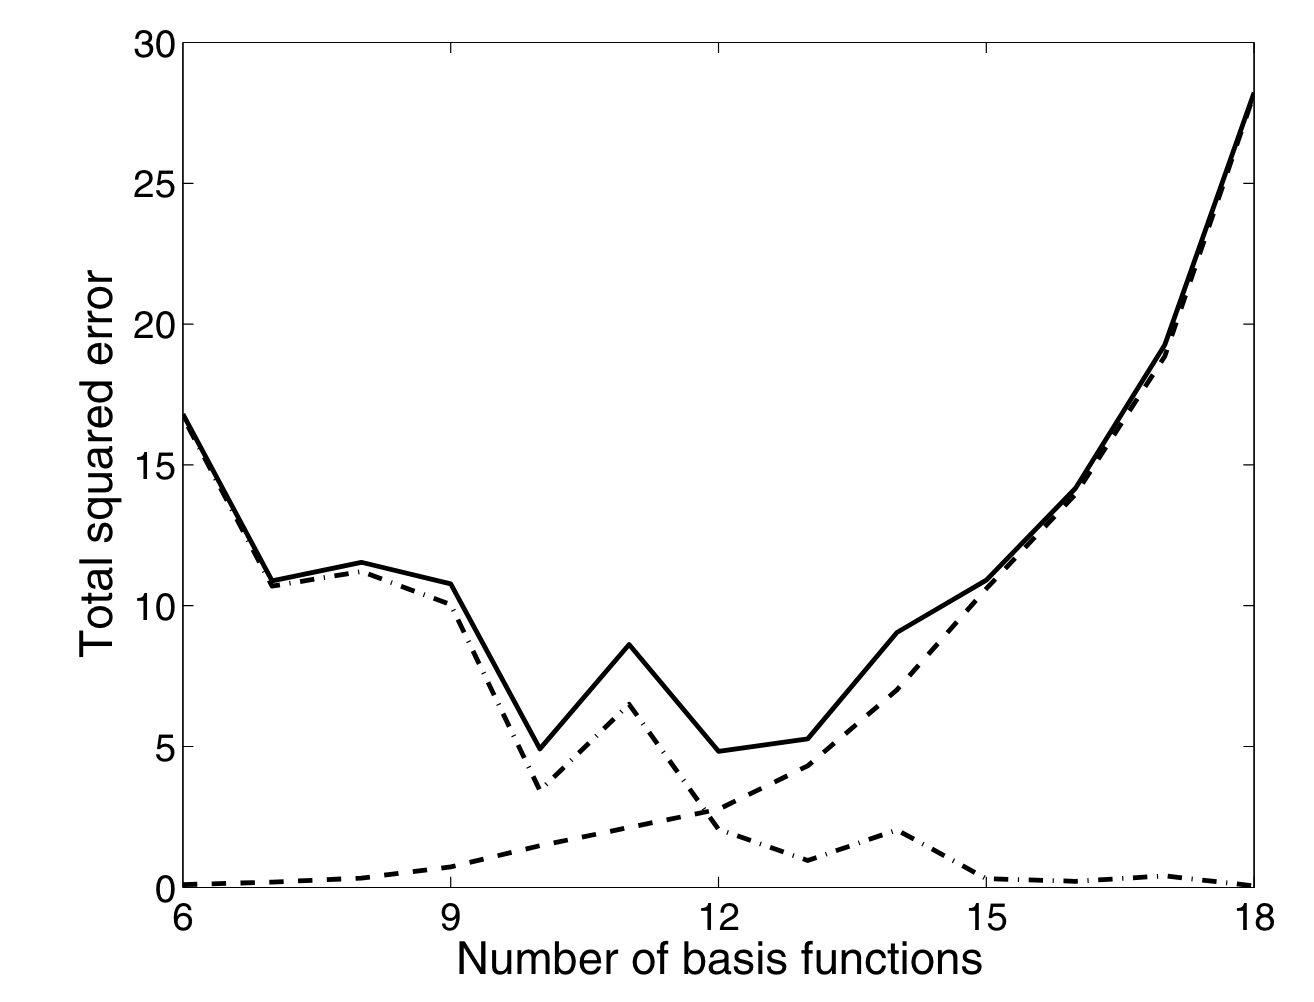
\includegraphics[width=0.5\textwidth]{Images/tradeoff.png}
\caption[Bias variance trade-off.]{The heavy solid line indicates mean squared error totaled across the ages of observation between three and sixteen. The dashed line shows the totaled sampling variance, and the dotted-dashed line shows the totaled squared bias \cite{ramsay_functional_2006}.}
\label{fig:tradeoff}
\end{figure}
\paragraph{Choose the right values of $\lambda$ in PENSSE.} When we have to decide which parameter to use to penalise \ref{eq:pensse}, we can carry out the same operation as in previous paragraph by minimising generalised cross validation defined as
\begin{equation}
\label{eq:gcv}
    \operatorname{GCV}(\lambda)=\left(\frac{n}{n-d f(\lambda)}\right)\left(\frac{\operatorname{SSE}}{n-d f(\lambda)}\right)
\end{equation}
where $df(\lambda)$ are the degrees of freedom value for the spline smooth and are computed as
\begin{equation}
   df(\lambda)=\operatorname{trace} \mathbf{S}_{\phi, \lambda}
\end{equation}
and $\mathbf{S}_{\phi, \lambda}$ is defined in \ref{eq:unbelcasino}.


\subsection{Functional Principal Component Analysis}
Functional principal component analysis (FPCA), which is nothing other than PCA applied to functional data, is a widely used technique when dealing with functional data. Indeed, when dealing with functional data, it is common practice to look for features that characterize typical functions. For example, we might be interested in the sinusoidal nature of periodic data \cite{ramsay_functional_2006}. When we talked about classical PCA, the linear combination consisted of a vector of weights and the observations of the dataset. In the case of FPCA, however, we have to translate this approach into the domain of functions, thus, into the domain of the "continuum". Thus, the \ref{eq:pcaf}, will become 
\begin{equation}
    f_i= \int \beta y_i = \int \beta(t) y_i(t) dt
\end{equation}
The weights $\lambda$ now become functions $\beta(t)$. 
\begin{figure}
    \centering
    \subfloat[\label{fig:mediafpca}]{
        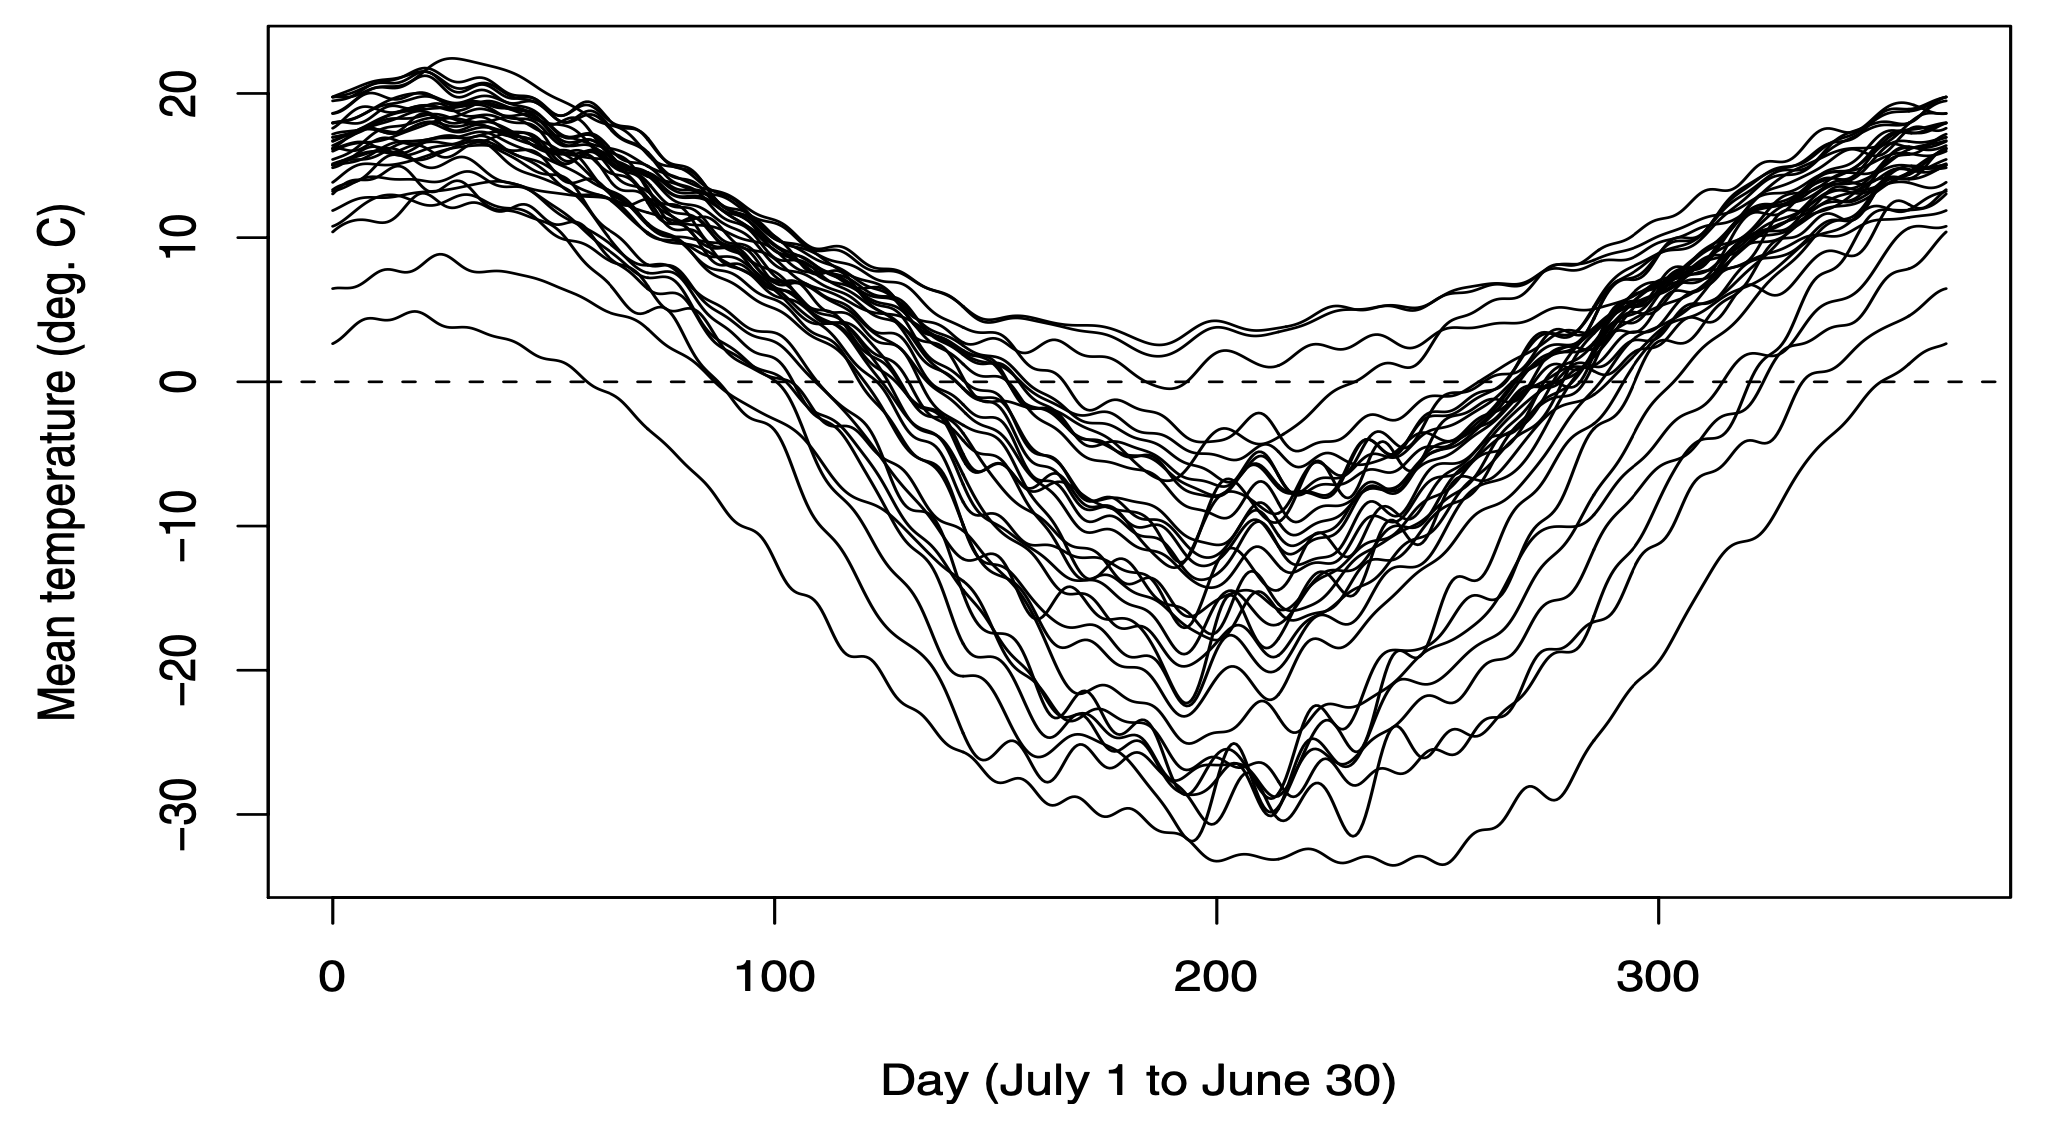
\includegraphics[scale=0.2]{Images/canadamedie.png}
    }
    \qquad
    \subfloat[\label{fig:canadapc}]{
        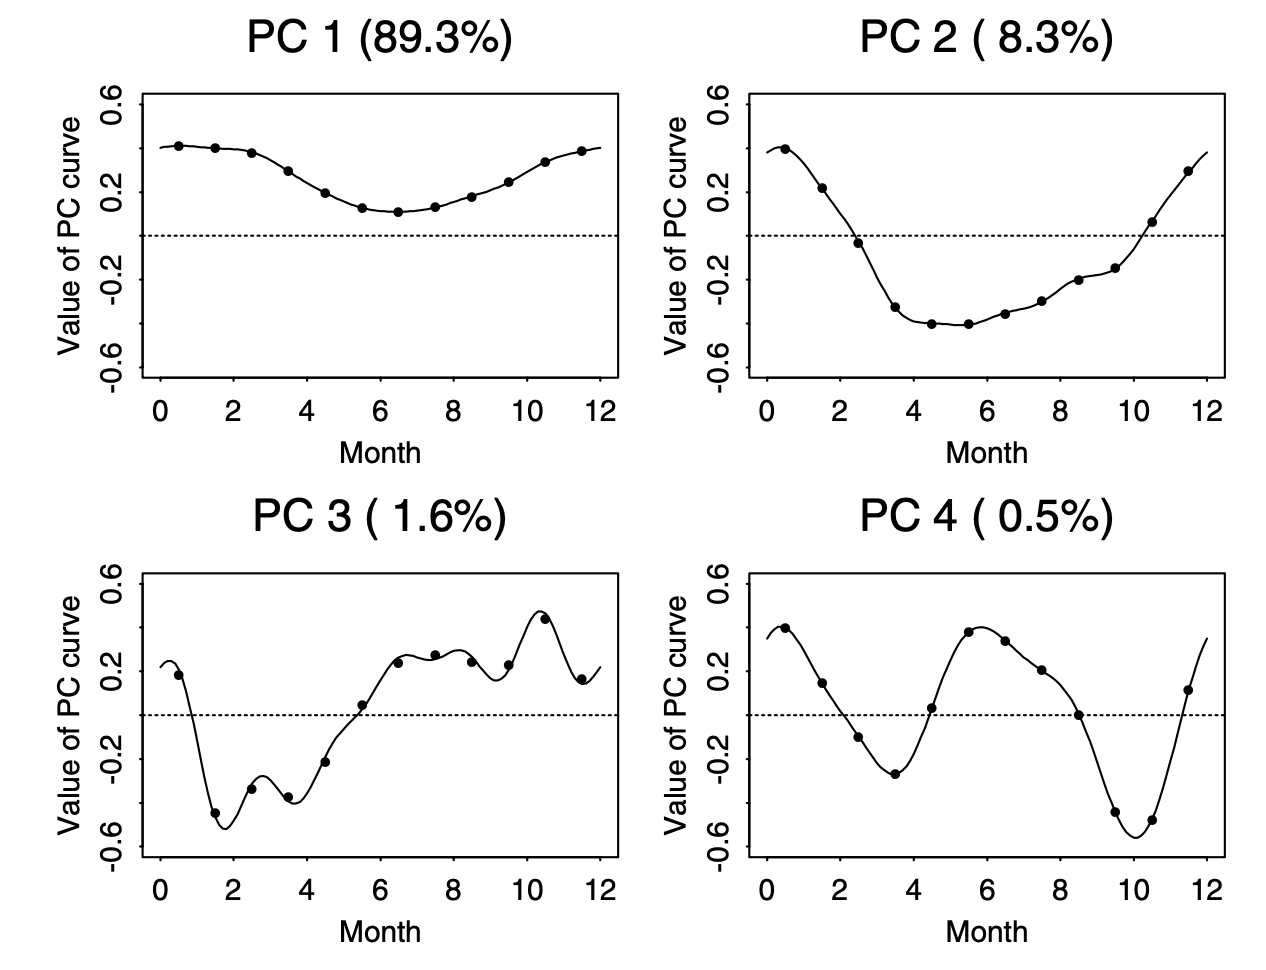
\includegraphics[scale=0.28]{Images/PCs.png}
    }
    \caption[Functional Principal Component Analysis.]{Mean temperature curve of the 35 different stations over the considered time period (a) and the first four PCs with relative proportion of explained variance (b) \cite{ramsay_functional_2006, ramsay_functional_2009}.}
    \label{fig:FPCA}
\end{figure}
As in PCA, each weight function has the task of capturing the greatest amount of variance and being orthogonal to all other weight functions. Thus, every weight function will have a decreasing associated amount of explained variance. For a more in-depth explanation of the calculation method, the reader can refer to \citeauthor{ramsay_functional_2006} (2006). Consider the example in Fig. \ref{fig:FPCA}.  The dataset consists of daily temperature data recorded at 35 locations in Canada from 1960 to 1994. Fig. \ref{fig:mediafpca} shows the 35 annual mean temperature curves. We can see that the first weight function, although always strictly greater than zero, has values in the winter months up to four times higher than in the summer months. Moreover, only the first PC explains 89.3\% of the total variance. This means that temperatures in the winter tend to be much more 'variable' than those in the summer. Thus, weather stations with high scores will have warmer than usual winters and warm summers, and the two highest scores are, in fact, assigned to Vancouver and Victoria on the Pacific Coast. On the other hand, the largest negative score goes to Resolute in the High Arctic. On the other hand, the second PC shows similar overall behavior to the first PC but is not strictly greater than zero. This means it corresponds to a measure of temperature uniformity throughout the year. For example, the highest score goes to Prince Roupert, a city on the Pacific coast, characterized by a slight temperature difference between the summer and winter. We can interpret each of the PCs just as in the PCA. However, as we can see from Fig. ef {fig:canadapc}, the third PC helps to explain only 1.6\% of the total variance, so it is much less significant.
% <<< End of Functional Data Analysis

%%%%%
%%%%%

% Bagging Voronoi Clustering Algorithm >>>
\section{Bagging Voronoi Classifier}
\label{sec:bvc}
\citeauthor{secchi_bagging_2013} (2013) presents the Bagging Voronoi Clustering Algorithm. It is an algorithm for unsupervised classification of functional data that exploits spatial dependence by repeatedly generating random connectivity maps and by clustering, at each replicate, local representatives of neighboring functional data. The algorithm is entirely non-parametric. Thus, we do not need any a priori data distribution hypothesis, making it more robust. The algorithm is structured in five consecutive steps. The first step involves using a Voronoi tessellation to partition the domain lattice. Voronoi diagram divides the plane into regions close to each object of a given set. In our case, these objects are just the sites of the lattice. We call these objects nuclei. Each nucleus has a corresponding region, called a Voronoi cell, consisting of all points of the plane closer to that nucleus than to any other. Let $X$ be a metric space and $d(\cdot, \cdot)$ be a distance function, in our case, Euclidean distance. Let $\Phi_n$ be the set of $n$ selected nuclei and let each nucleus be a tuple of coordinates $\left(P_k\right)_{k\in \Phi_n}$. The formal definition of a Voronoi cell $R_k$ associated with the site $P_k$ is 
\begin{equation}
    \label{eq:voronoicell}
    R_k=\{x\in X \mid d(x, P_k)\leq d(x, P_j),\forall j\neq k\}
\end{equation}
The Voronoi tessellation is the collection of all the cells in the space.
Fig. \ref{fig:voronoi} shows an example.
\begin{figure}
    \centering
    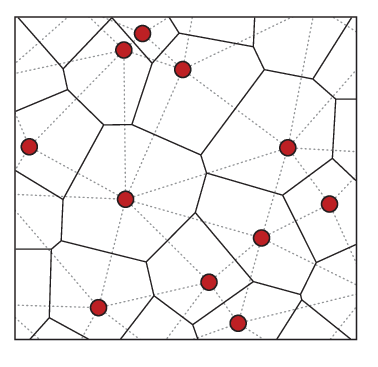
\includegraphics[width=0.3\textwidth]{Images/A-set-of-atoms-the-associated-Voronoi-tessellation-solid-lines-and-the-Delaunay.png}
    \caption[Voronoi tessellation.]{Example of Voronoi tessellation with highlighted nuclei.}
    \label{fig:voronoi}
\end{figure}


\subsection{Algorithm Steps}
\label{subsec:algsteps}
This section describes in detail the algorithm steps. In Alg. \ref{alg:bvc}, there is the pseudo-code of the Bagging Voronoi algorithm. Suppose a latent field of labels $\Lambda_0:\mathcal{S}_0 \rightarrow \{1,\dots,L\}$ which is defined on the lattice $\mathcal{S}_0$. $\Lambda_0(\mathbf{x})$ is the true unknown label associated to the site $\mathbf{x}\in\mathcal{S}_0$, where $\mathcal{S}_0 \subset \mathcal{S}$ and $\mathcal{S}$ is a measurable subset of $\mathbb{R}^d$. In addition, suppose that a functional datum is observed in each site $\mathbf{x}\in\mathcal{S_0}$. The steps needed to find an estimation of true label $\Lambda_0(\mathbf{x})$ the following steps are needed.

\begin{algorithm}
\scriptsize
    \caption{\footnotesize{Bagging Voronoi Classifiers}}
    \label{alg:bvc}
    \begin{algorithmic}
    \STATE \textbf{Bootstrap:}
    \STATE Initialize $B, n, p, K$. Choose a metric $d(\cdot,\cdot).$
    \FOR{$b:=1$ to $B$}
    \STATE{Randomly generate a set of nuclei $\Phi^b_n=\{\mathbf{Z}_1^b, \dots, \mathbf{Z}_n^b\}$ among the sites in $\mathcal{S}_0$}
    \FOR{$i=1$ to $n$}
    \STATE $\mathbf{Z}_i^b\sim\mathcal{U}(\mathcal{S}_0)$, where $\mathcal{U}$ is the uniform distribution on the lattice. Obtain a random Voronoi tessellation of $\mathcal{S}_0, \{V(\mathbf{Z}_i^b|\Phi_n^b\}^n_{i=1}$ by assigning each site $\mathbf{x}\in \mathcal{S}_0$ to the nearest nucleus $\mathbf{Z}_i^b$, according to the specified distance $d(\cdot,\cdot).$
    \ENDFOR
    \FOR {$i:=1$ to $n$}
    \STATE Compute the function $g_i^b$, acting as local representative, by summarizing information carried by the functional data associated to sites belonging to the $i$-th element of the tessellation $V(\mathbf{Z}_i^b|\Phi_n^b)$.
    \ENDFOR
    \STATE Perform dimensional reduction of the local representatives $\{g_1^b,\dots, g_n^b\}$ by projecting them on the space spanned by a proper $p$-dimensional scores vectors $\{\mathbf{g}_1^b,\dots, \mathbf{g}_n^b\}$, which are then clustered in $K$ groups according to suitable unsupervised method.
    \ENDFOR
    \STATE \textbf{Aggregation:} perform cluster matching
    \FOR {$k:=1$ to $K$}
    \FOR {$b:=1$ to $B$}
    \STATE indicate with $C_k^b$ the set of $\mathbf{x} \in \mathcal{S}_0$ whose label is equal to $k$, and match the cluster labels across bootstrap replicates, to ensure identifiability.
    \ENDFOR
    \ENDFOR
    \FOR {$\mathbf{x} \in \mathcal{S}_0$}
    \STATE Calculate the frequencies of assignment of the site to each of the $K$ clusters along iterations, \textit{i.e.}, $\pi_{\mathbf{x}}^k=\#\{b\in\{1,\dots,B\}:\mathbf{x}\in C_k^b\}/B, \forall k=1,\dots,K$
    \ENDFOR
    \end{algorithmic}
\end{algorithm} 


\paragraph{Step 1: Voronoi Tessellation.} Select a set of points $\mathbf{x}\in\mathcal{S}$ as nuclei for the Voronoi tessellation. Thus, let $\Phi_n=\{\mathbf{Z}_1, \dots, \mathbf{Z}_n\}$ be the set of $n$ points in $\mathcal{S}$ sampled from a proper distribution $F$ defined on S: this will be the set of nuclei of the Voronoi tessellation. For each $\mathbf{Z}_i\in\Phi_n$ define the polyhedron
\begin{equation}
    \label{eq:polyedron}
    V\left(\mathbf{Z}_i \mid \Phi_n\right)=\{\mathbf{x}\in\mathcal{S} : d\left(\mathbf{x},\mathbf{Z}_i\right) \leq d\left(\mathbf{x}, \mathbf{Z}_j\right), \quad \text{for all}\quad \mathbf{Z}_j \in \Phi_n, i\neq j\}
\end{equation}
to be the closest Voronoi cell with nuclues $Z_j$ for the Voronoi tessellation induced by $\Phi_n$.
\paragraph{Step 2: Functional Local Representatives.} Consider $T$, a bounded interval of $\mathbb{R}$ and a realization $f_{\mathbf{x}}:T\rightarrow \mathbb{R}$ of a functional random variable is observed in each site $\mathbf{x}$ of the lattice $S_0$. The Voronoi tessellation of the lattice $S_0$ computed in the previous step, defines random neighborhoods. For each element $V_i$ of the Voronoi tessellation, we sum up the information contained in the sub-sample $\{f_{\mathbf{x}}\}_{\mathbf{x} \in V_i}$ by estimating a functional local representative through a method that exploits spatial dependence of neighboring data. For example, the authors suggest using a weighted mean with a Gaussian kernel. Still, we can use any functional local representative we prefer, depending on our needs and problem domain. For $i=1, \dots, n$ the functional local representative $g_i$ aforementioned is defined as
\begin{equation}
    \label{eq:gaussianmean}
    g_i(t)=\frac{\sum_{\mathbf{x}\in V_i}w^i_{\mathbf{x}}\cdot f_{\mathbf{x}}(t)}{\sum_{\mathbf{x}\in V_i}w^i_{\mathbf{x}}}
\end{equation}
where $w_{\mathbf{x}}^i$ is a Gaussian weight centered in $Z_i$ and decreasing with respect to $d\left(\mathbf{x}, \mathbf{Z}_i\right)$. Intuitively, we assume that spatial dependence between two sites decreases when the distance between them increases. The kernel covariance matrix is $\sigma^2\mathbb{I}_2$, where $\sigma=d_{max}/d_{min}$, being $d_{max}$ and $d_{min}$ the maximum and minimum distance between two nuclei of the tessellation, respectively. This choice connects $\sigma$ to the mean dimension of the tessellation via an estimator of the element's mean diameter. The choice of $n$, which sets the tessellation dimension and thus the number of local representatives to be computed, greatly influences the algorithm behavior: in general, we have to find an optimal $n$ such that we find a good compromise between variance and bias. We will see two possible approaches for choosing the optimal $n$ value in Section \ref{sec:irradiance}.
\paragraph{Step 3: Dimensional Reduction and Clustering} The algorithm's third step aims to perform data dimensional reduction and cluster the dimensionally reduced data. The most common tool used for dimensionality reduction of functional data is FPCA. For dimensional reduction of functional data, we need to find the best projection local representatives $\{g_1, \dots, g_n \}$ onto the space generated by a proper functional basis of finite dimension $p$. To choose the correct dimension $p$, we can use the amount of variance explained by each functional principal component. "For instance, we could set a threshold, say 95\%, and keep the first $p$ principal components that account for a variance greater than or equal to 95\% of the total variance of the initial functional data. Alternatively, we could use the scree plot of the absolute variance explained by each principal component and retain the $p$ components before the knee. This latter approach offers more freedom of choice to the analyst. Thus, a deep understanding of the problem domain becomes essential. Using a bootstrapping method, we can repeat steps 1-3 $B$ times, where $B$ is arbitrarily chosen. 
\paragraph{Step 4: Cluster Matching} The output of the $b$-th replicate of the bootstrap phase of the algorithm is a label assignment for each local representative estimated during the $b$-th run. All sites $\mathbf{x} \in V_i^b$ get the same label associated with the function local representative $g_i^b(t)$. To obtain a classification map of the lattice $\mathcal{S}_0$, we consider the frequency distribution of assignment of each site to each of the $K$ clusters along the $B$ replicates. To compute this frequency distribution, we need, in turn, to assume that cluster labels $\{C_1^b, \dots, C_K^b\}$ are coherent along the $B$ replicates. More specifically, we want cluster labels $\{C_1^b, \dots, C_K^b\}$ to be coherent with $\{C_1^m\, \dots, C_K^m\}$, for all $m<b$ and $b\geq2$. This is obtained through cluster matching. Cluster matching is a set of techniques that allow us to keep different clustering algorithm outputs coherent. I will discuss a simple approach based on a contingency table. The algorithm looks for the label permutation that minimizes the total sum of the off-diagonal frequencies in the contingency table describing the joint distribution of sites along the classifications at two subsequent replicates. At the end of clustering matching, for each site $\mathbf{x}$ we will have a vector $\pi_{\mathbf{x}}^K=\left(P_1, \dots, P_K\right)$ where each $P_i, \quad i=1,\dots,k$ is the frequency the label $k$ was assigned to the site $\mathbf{x}$. The final label will be the label associated with maximum $P_k$. In other words, it is a majority voting process among the different replicates $b$.
\paragraph{Step 5: Output Evaluation} To have an overview of the statistical validity of the clustering just performed, we can use \textit{spatial entropy}. This concept is directly derived from the classical notion of entropy. Considering the frequency distribution vector $\boldsymbol{\pi}=(\pi_{\mathbf{x}}^1,\dots,\pi_{\mathbf{x}})^K$ of each site $\mathbf{x} \in \mathcal{S}_0$ to each of the $K$ clusters obtained after the bootstrapping step of the algorithm. The entropy associated site $\mathbf{x}$ classification in the site $\mathbf{x}\in\mathcal{S}_0$ is defined as
\begin{equation}
\mathbf{\eta}_{\mathbf{x}}=-\sum_{k=1}^K\pi_{\mathbf{x}^k}\cdot \log(\pi_{\mathbf{x}^k})
\end{equation}
which assumes the minimum value 0 when there is an $r$ such that $\pi_{\mathbf{x}}^r=1$ while $\pi_{\mathbf{x}}^k=0$ for all $k\neq r$ and maximum value $\log(K)$ when $\pi_{\mathbf{x}}^k=\frac{1}{K}$ for $k\in\{1,\dots,K\}$. We can see spatial entropy as a measure of the disorder of the frequency of assignment the site $\mathbf{x}\in\mathcal{S}_0$ to cluster $k$. Moreover, we can compute the \textit{average normalized entropy} to have a global evaluation index of the clustering performed. Average normalized entropy is defined as
\begin{equation}
\label{eq:avgentropy}
    \eta^K=\frac{\sum_{\textbf{x}\in\mathcal{S}_0}\eta_{\mathbf{x}}^K}{\log(K)\cdot |\mathcal{S}_0|}
\end{equation}
From \ref{eq:avgentropy} we can appreciate how the index has been normalized to maximum value $\log(K)$ in order to allow comparison over different choices of $K$. An other possible index for evaluating a classification in the ratio
\begin{equation}
    \label{eq:theta}
    \theta=\frac{tr(B)}{tr(B)+tr(W)}
\end{equation}
where $B$ and $W$ are the final between and within cluster sum of squares matrix, respectively. This index can be seen as the percentage of variance explained by splitting the observations in clusters.
% <<< End of Bagging Voronoi Clustering Algorithm

%%%%%
%%%%%

% Succesful case of the algorithm >>>
\section{Clustering of Irradiance Data}
\label{sec:irradiance}
In this section, we will discuss an examples of how the algorithm outlined in the previous paragraph has been successfully applied in clustering of irradiance data performed in \citeauthor{secchi_bagging_2013} (2013). This section addresses any potential questions or uncertainties the reader may still have regarding the use of Algorithm \ref{alg:bvc}. 

Insolation refers to the amount of solar radiation energy captured on a specific surface area over a set time period. Typically, it is computed as average irradiance in kilowatt-hours per square meter per day (\unit{\kilo\watt.h/\metre^2.day}). The authors focused on direct insolation, which pertains to the solar irradiance measured at a particular location on Earth with a surface facing directly toward the sun's rays, omitting diffuse insolation. Diffuse insolation refers to the solar energy scattered or reflected by atmospheric components overhead. The value of direct insolation is derived from the solar constant minus the atmospheric reductions from absorption and scattering. While the solar constant is influenced by factors like Earth's distance from the sun and solar cycles, the losses are contingent on factors such as the time of day (which affects the light's path through the atmosphere based on the sun's elevation angle), cloud coverage, atmospheric moisture, and other contaminants. The authors' goal was to identify areas of the planet that are optimal with respect to the positioning of solar power collectors by considering parameters that depend on direct insolation. The data available for the analysis consists of vectors in $\mathbb{R}^{12}$ indexed by each site of the lattice. Sites are located on a non-uniform lattice $\mathcal{S}_0=\bigcup_{\lambda \in Z_{\mathbf{1}};\theta \in Z_{\mathbf{2}}}A_{\lambda\theta}$ where $Z_{\mathbf{1}} = \{ -180, -179, \dots, 178, 179\}$ and $Z_{\mathbf{2}} = \{ -66, -65, \dots, 65\}$: each element $A_{\lambda\theta}$ is the portion of the earth surface which is included between the meridians at longitude $\lambda$ and $\lambda + 1$ in degrees, and between the parallels at latitude $\theta$ and $\theta + 1$ in degrees. This lattice is, of course, non-uniform and includes 47,520 worldwide non-polar districts. In each site, the 12 measures correspond to the monthly maximum energy deficit values with respect to the monthly average. The maximum and average values are computed over the 22-year period from July 1983 to June 2005. For each site, authors obtained a functional datum $Y_{\lambda,\theta}(t)$ by smoothing $\{Y_{\lambda\theta}^1, \dots, Y_{\lambda\theta}^12\}$ with a Gaussian kernel with bandwidth equal to 1.5, where $Y_{\lambda\theta}^\nu$ is the irradiance data for each month. The authors used a Gaussian isotropic kernel to compute the weighted average local representatives. They selected the first $p=3$ functional principal components since with only these three components, the proportion of explained variance was more than 95\%. For classifying the scores of the $n$ representatives, they employed the K-Means algorithm with the $L^2$ semi-metric induced by the principal components.
\begin{figure}
    \centering
    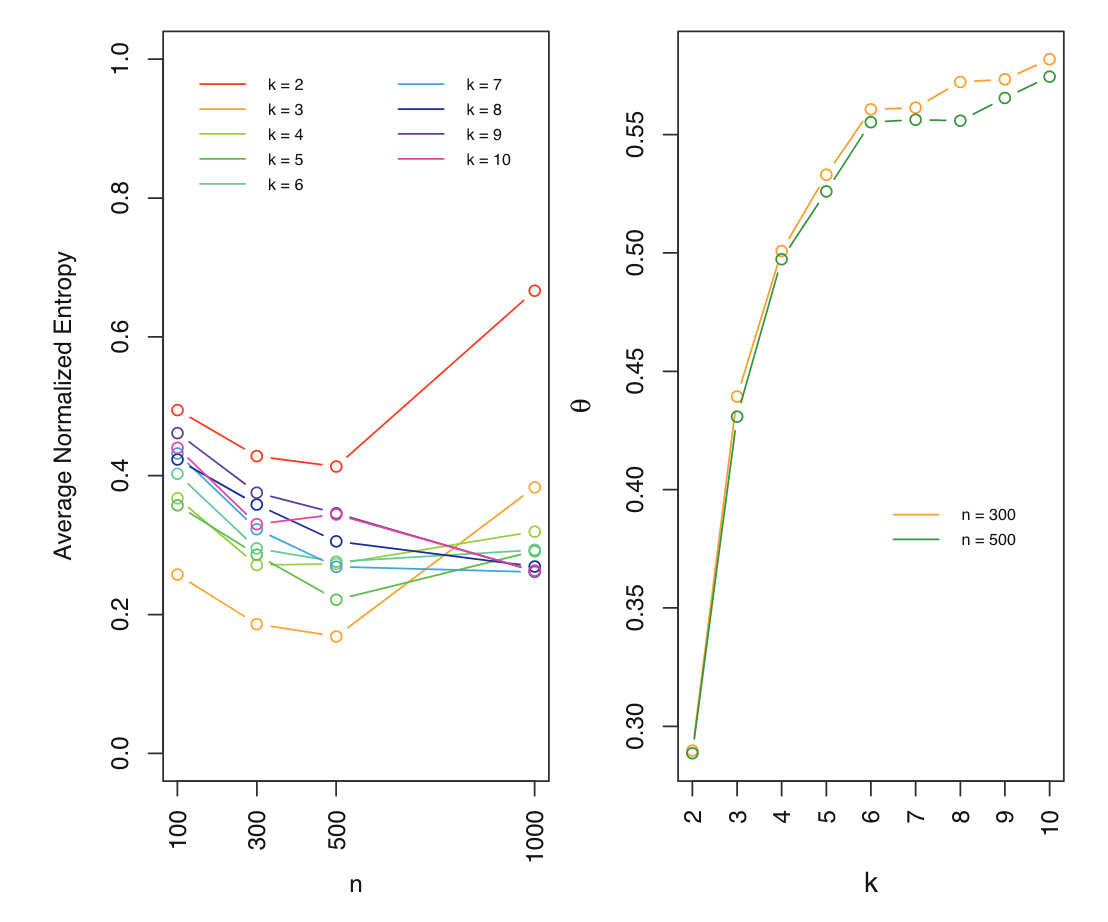
\includegraphics[scale=0.5]{Images/baggingscreeplot.png}
    \caption[Result on irradiance data.]{Algorithm performances with irradiance data. On the left, average normalized entropy, on the right the index $\theta$ \cite{secchi_bagging_2013}.}
    \label{fig:baggingscreeplot}
\end{figure}
Subsequently, as with all classical clustering problems, they performed the clustering multiple times to obtain the scree plot shown in Fig. \ref{fig:baggingscreeplot} and to select the optimal number of clusters, $K$. With this specific algorithm, it was also necessary to determine the optimal number of nuclei, $n$, for the initial Voronoi tessellation. To find the scree-plots shown in Fig. \ref{fig:baggingscreeplot}, the number of bootstrap replications was set at $B=100$, and the parameters $n$ and $K$ were varied. The optimal choice for these two parameters was made using average normalized spatial entropy, the index $\theta$, and the normalized spatial entropy map in conjunction. Starting from the scree-plot of average normalized entropy in Fig. \ref{fig:baggingscreeplot}, we can see that for $n=500$, we have two local minima, specifically for $K=3$ and $K=5$. From the same figure, we can observe that the graph of $\theta$ suggests that the number of clusters $K=6$ appears to be the most reasonable. Indeed, using $K=7$ would not be a good choice, as it would not enhance the classification obtained. Consequently, the classification should yield good results for $K=5$ and $K=6$. This was also confirmed by the maps of the normalized entropy, shown in Fig. \ref{fig:irrentropy}.
\begin{figure}[H]
    \centering
    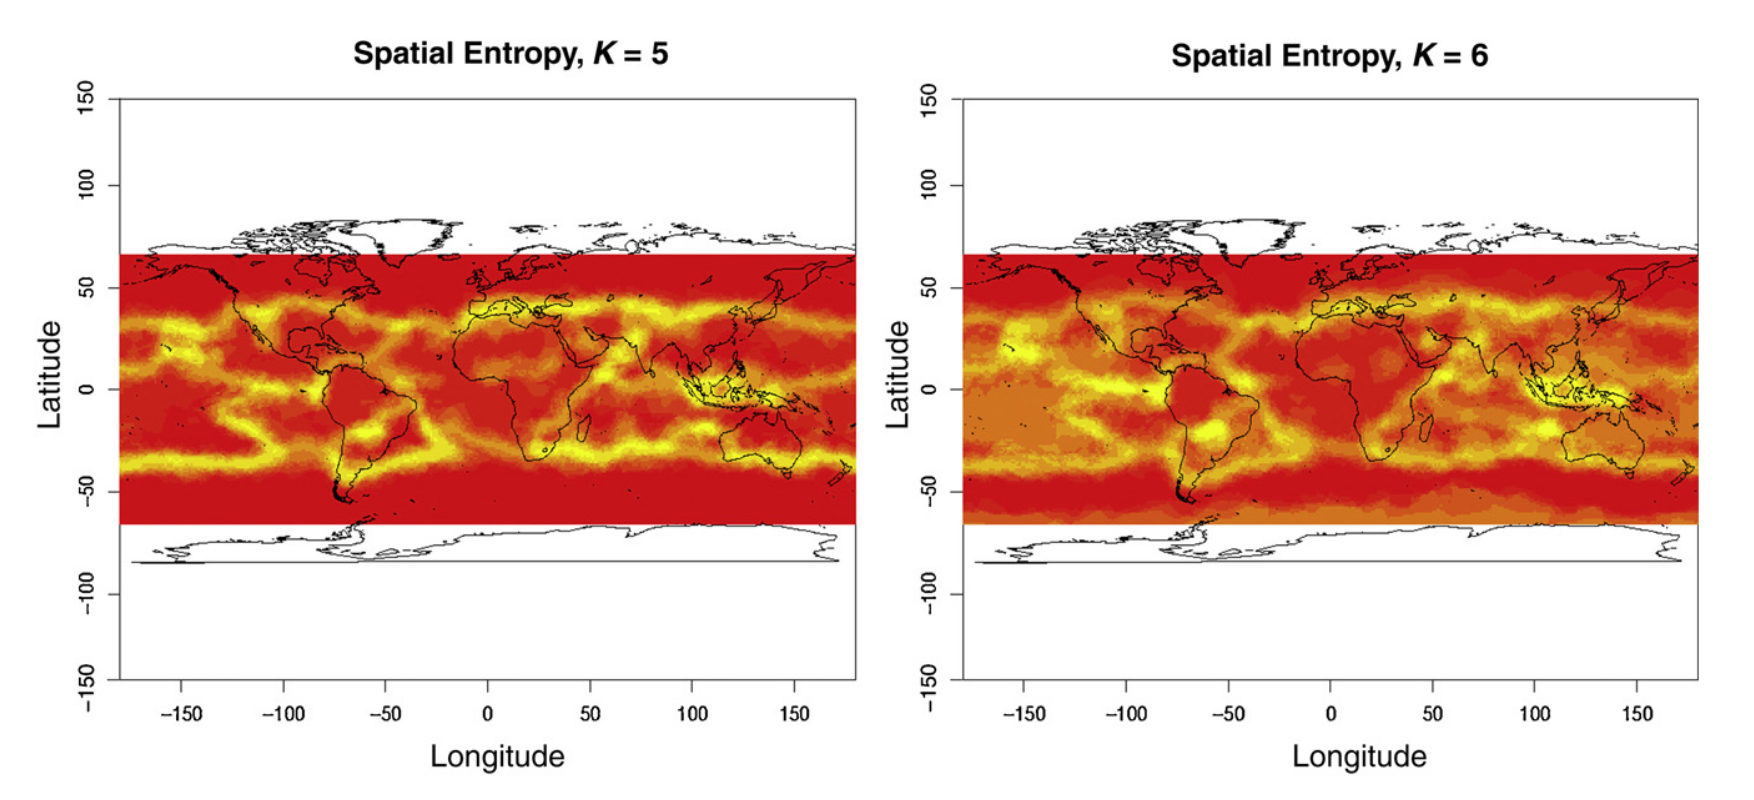
\includegraphics[scale=0.5]{Images/irrentropy.png}
    \caption[Spatial entropy for irradiance data.]{Normalized spatial entropy maps associated to the classification with K = 5 (left) and K = 6 (right). Colors from red to white correspond to values from 0 to 1; higher values identify areas where classification is more uncertain. \cite{secchi_bagging_2013}.}
    \label{fig:irrentropy}
\end{figure}
The final choice $K=5$ was made looking at maps in Fig. \ref{fig:irrentropy}, which tell us that for $K=5$ the classification is more robust, and from the fact that with $K=5$, the algorithm identified different homogeneous macro-areas which seem interpretable in terms of the observed phenomenon. In Fig. \ref{fig:resbagging}, there is the final classification for irradiance data. The two classifications are not in contrast but somehow support each other. As mentioned earlier, we can take advantage of the functional nature of the data to derive additional insights that wouldn't be possible with traditional clustering algorithms. For instance, the red cluster exhibits a non-seasonal pattern that remains consistent throughout the year, and the green and yellow clusters have opposite seasonal patterns. The advantage of using $K=6$ is that we can identify some sites characterized by a very high seasonality with the orange cluster. To conclude, it's noteworthy that spatial entropy is systematically higher near the boundary between two clusters. This is because the functional data is actually spatially dependent, and hence data near the boundaries are more challenging to cluster.
\begin{figure}
    \centering
    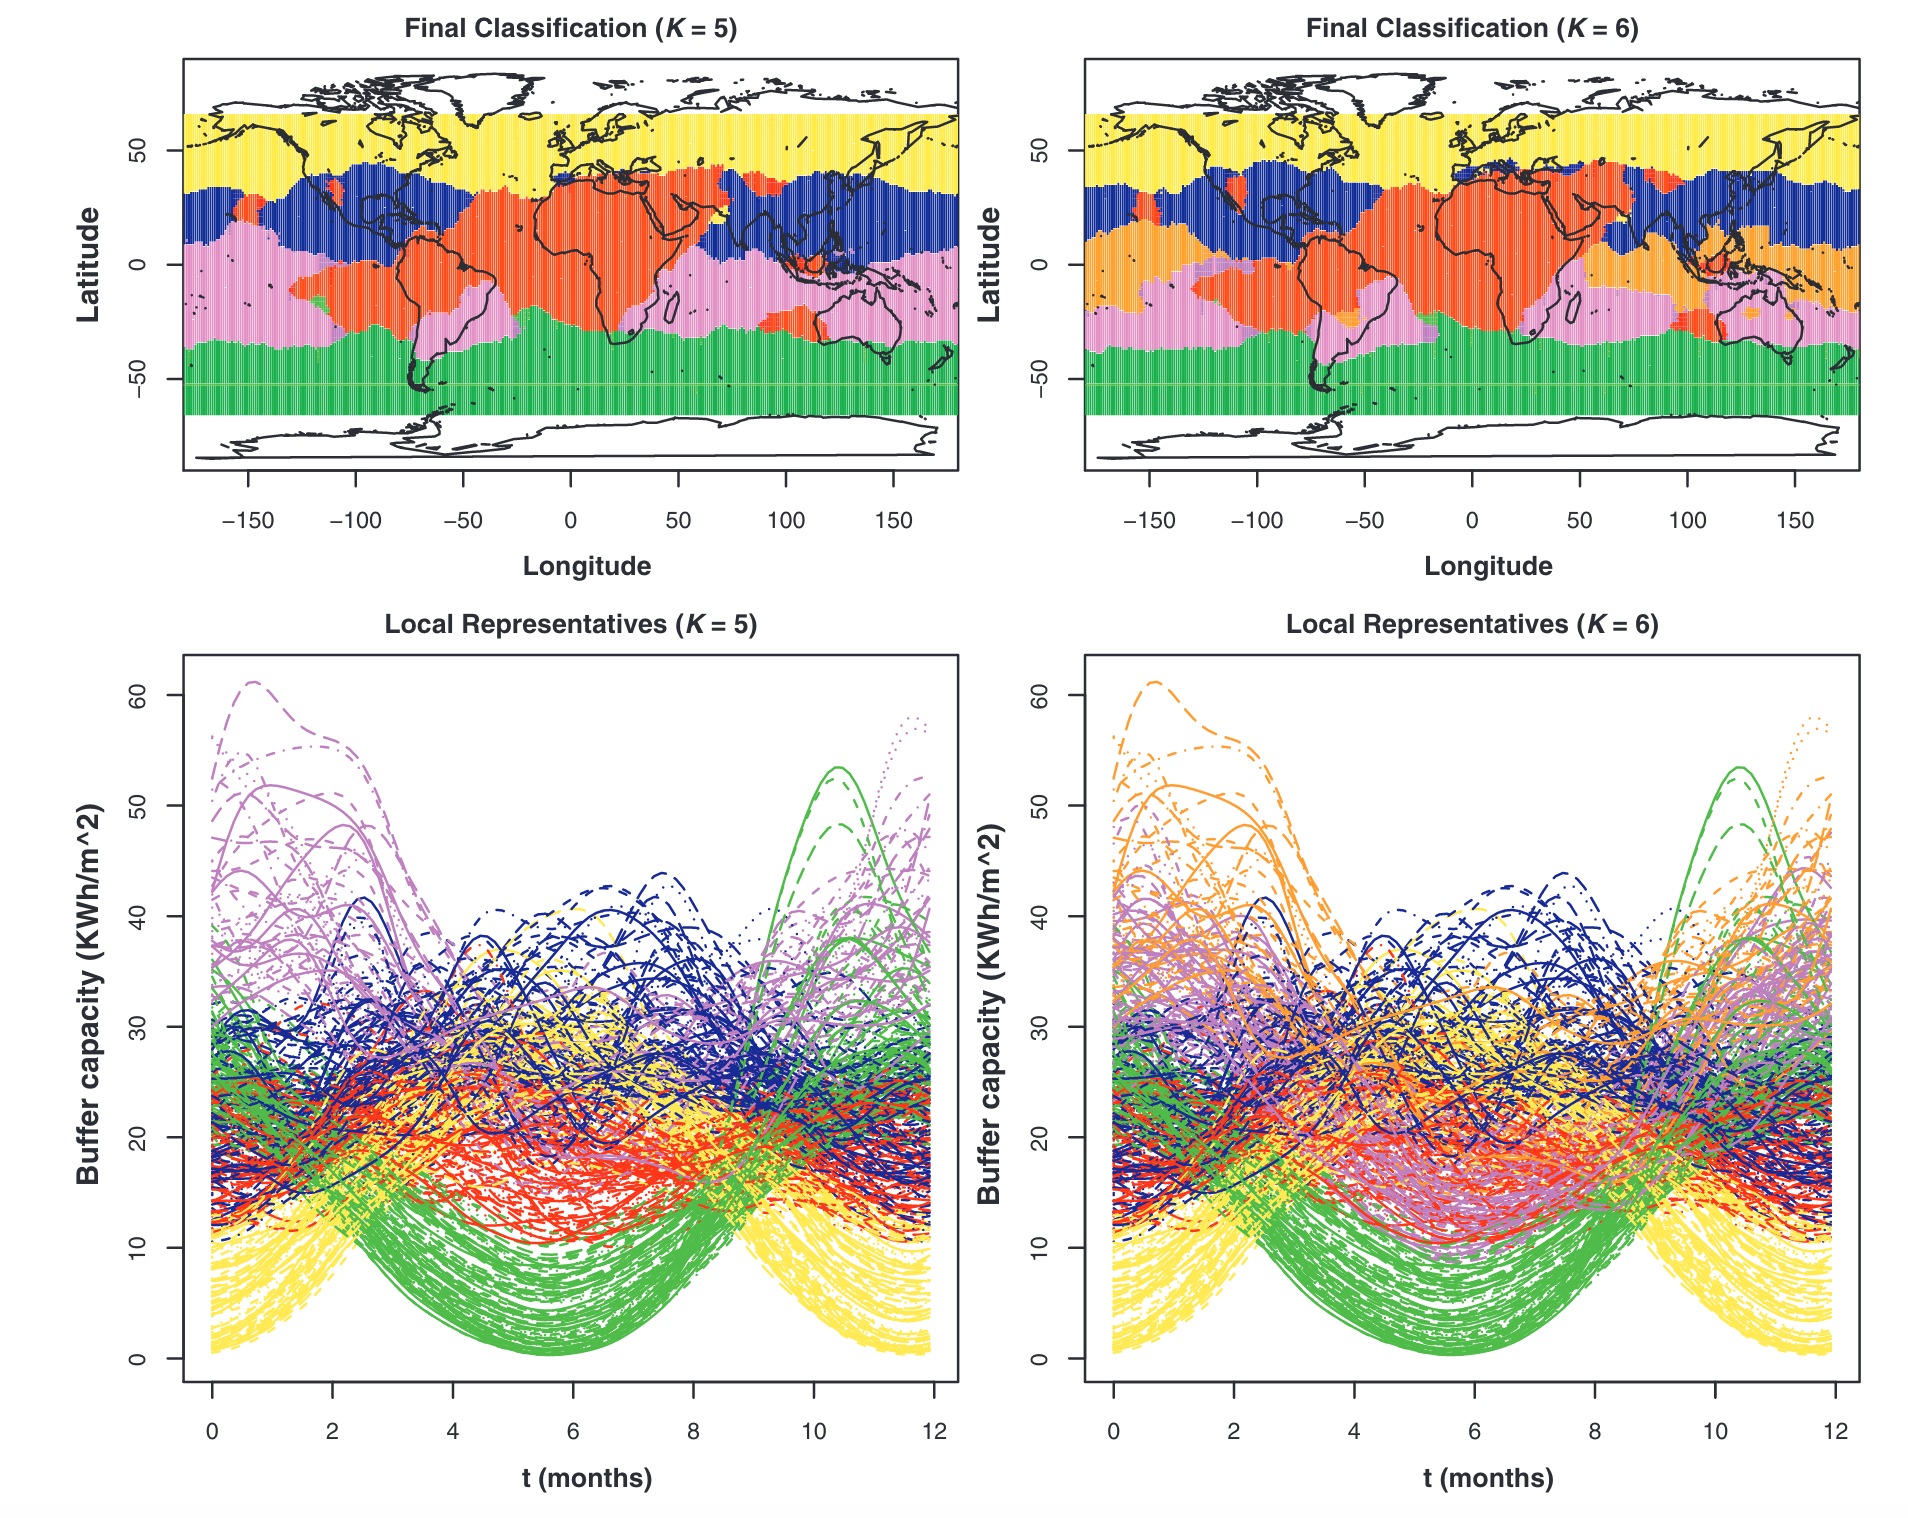
\includegraphics[scale=0.4]{Images/resbagging.png}
    \caption[Classification of irradiance data.]{In the top panels, final classification maps obtained via a majority vote on frequencies of assignment, and by setting $K = 5$ (left) or $K = 6$ (right).In the bottom panels, a set of functional local representatives obtained with $n = 500$ in one of the iterations of the algorithm and clustered with $K = 5$ (left) and with $K=6$ (right). From \citeauthor{secchi_bagging_2013} \citeyear{secchi_bagging_2013}.}
    \label{fig:resbagging}
\end{figure}
The parallelism between irradiance data/planet and temperature profiles/print area seems straightforward and relatively clear. So, it's reasonable to believe that an application in additive manufacturing could lead to positive results.

%\subsection{Analysis of Spatio-Temporal Mobile Phone Data in Milan}
% \label{subsec:mobilephonemilan}
% I have chosen to present this example to illustrate to the reader the flexibility of the previously discussed algorithm. It demonstrates how the method can adapt to different data dimensionality reduction techniques and how a Fourier basis can represent functional data exhibiting certain seasonality, as with lattice structures in Section. \ref{subsec:devcell}.
% In \citeauthor{secchi_analysis_2015} \citeyear{secchi_analysis_2015}, authors examined high-dimensional, geo-referenced mobile phone usage data from Milan's urban area to discern activity patterns within the city over time. The goal was to identify specific urban zones with similar temporal patterns, which could indicate specific activities or events in those areas. To achieve the goal, they decided to use the algorithm explained in Section \ref{sec:bvc} coupled with treelet analysis (I'll explain it in just a moment). 
% The data available for analysis are from Telecom Italia. In this dataset, the metropolitan city of Milan is divided into a uniform lattice $\mathcal{S}_0$ consisting of 97x109 sites. In each location, the average number of mobile phones simultaneously using the network for calling is provided every 15 minutes over 14 days.

% %%%%% Grammarly eseguito sul testo qua sopra ^^^


% This quantity is called Erlang and it is defined as
% \begin{equation}
%     \label{eq:erlang}
%     E_{\mathbf{x}j}=\frac{1}{15}\sum_{q=1}^Q \left| T_{\mathbf{x}j}^q \right|
% \end{equation}
% where $T_{\mathbf{x}j}^q$ indicates the time interval in which the $q$-th mobile phone is using the network for calling while moving within site $\mathbf{x}$ and during the $j$-th quarter of an hour. The Erlang data was recorded every quarter of an hour, from March 18th, 2009, 00:15, till March 31st, 2009, 23:45. Fig. \ref{fig:secchino} there is an example of an Erlang profile.
% \begin{figure}[H]
%     \centering
%     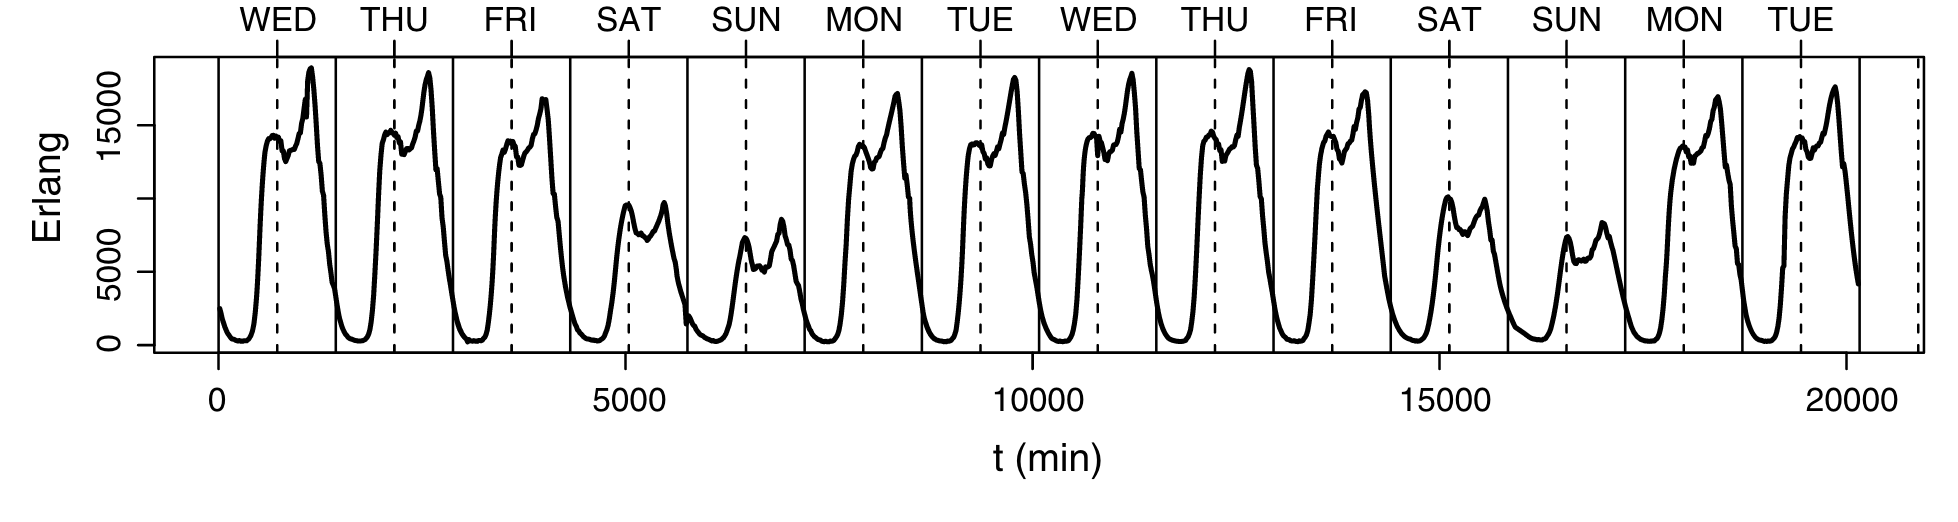
\includegraphics[scale=0.43]{Images/secchierlang.png}
%     \caption[Erlang profile.]{Erlang profile for a site in the lattice $\mathcal{S}_0$ \cite{secchi_analysis_2015}.}
%     \label{fig:secchino}
% \end{figure}
% However, for some sites of the lattice, Erlang profiles had some missing values, and in some instances, they were entirely missing. Therefore, after the data cleaning phase, the authors decided to focus only on a non-uniform time grid of $p = 1,308$ elements, each element of the time grid being relative to a quarter of an hour for which an Erlang measurement has been observed in at least one site of the lattice. In Algorithm \ref{alg:bvc} for dimensional reduction of functional data, FPCA was suggested. While FPCA stands as an effective technique for identifying optimal subspaces to represent data, it has a limitation in its global approach, making it less appropriate for multi-resolution analysis. This is primarily because its basis elements typically involve a linear combination of all foundational variables. So, authors decided to use a treelet basis, introduced in \citeauthor{lee_treeletsadaptive_2008} (2008). For this specific case, since the data exhibits an evident seasonality, authors decided to use a Fourier basis with a period equal to 1 week. Thus, the reconstructed functional form of the Erlang profile for site $\textbf{x} \in \mathcal{S}_0$ is a function $E_{\textbf{x}(t)}$ such that:
% \begin{equation}
%     E_{\textbf{x}}(t)=\frac{c_0^{\textbf{x}}}{2} + \sum_{h=1}^H \left[a_h^{\textbf{x}}\cos \left( h\omega t\right) + b_h^{\textbf{x}}\cos \left( h\omega t\right) \right]
% \end{equation}
% where $t \in \left[ 0; T\right]$, $\omega = 2\pi/T$ and $T=60 \times 24 \times 7$ is the period expressed in minutes. To choose the optimal basis dimension $H$, we can use the power spectrum associated to the site~-~wise smoothing of the Erlang data with a Fourier basis of large dimension $H = 200$. The power spectrum of the Fourier expansion of a signal represents the amplitude of the signal as a function of the frequency, and at the $h$-th frequency it is related to the amplitude of the $h$-th harmonic

% \begin{equation}
%     \label{eq:spectrum}
%     P_{\mathbf{x}}(h)=\sqrt{(a^{\mathbf{x}}_h)^2 + (a^{\mathbf{x}}_h)^2}
% \end{equation}

% Thus, the more the $h$-th harmonic is relevant in the explanation of features occurring in the data, the more $P_{\mathbf{x}}(h)$ will be large. From the spectrum in Fig. \ref{fig:fantasmino}, we can see that local maximum happening at multiple of 7 (the dotted lines), while for $H >100\omega$, power spectre becomes almost negligible.

% \begin{figure}[H]
%     \centering
%     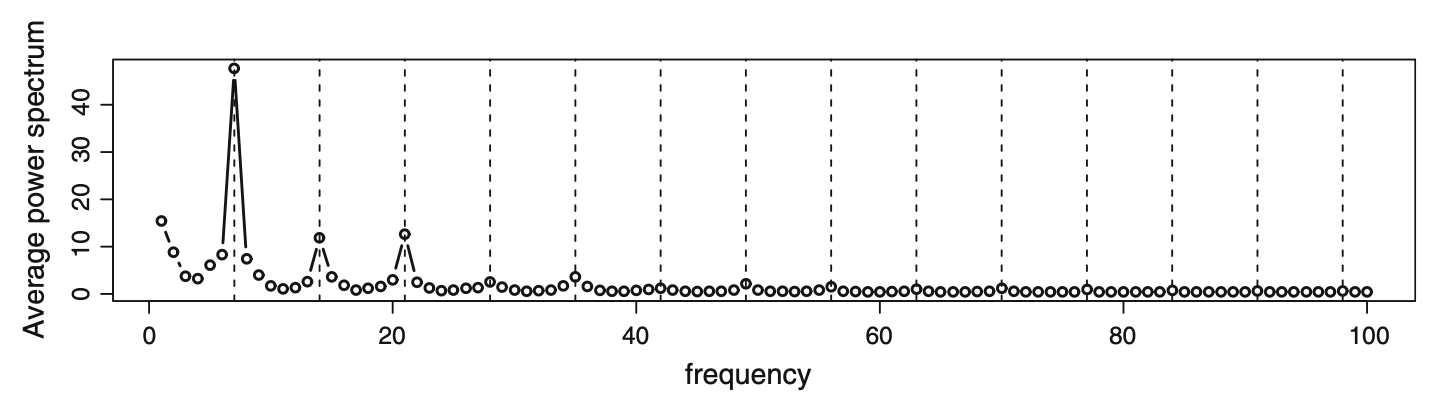
\includegraphics[scale=0.6]{Images/fantasmino.png}
%     \caption[Spectrum of Erlang data.]{Average power spectrum $P(h)$ obtained via site-wise smoothing of the Erlang measures with a Fourier basis of dimension $H = 200$. Only the values of $P(h)$ for$ h = 1, \dots, 100$ are shown in the plot. Dotted vertical lines are drawn for multiples of 7 \cite{secchi_analysis_2015}.}
%     \label{fig:fantasmino}
% \end{figure}

% As did in Section , the metric $d(\cdot, \cdot)$ used is Euclidean distance, the total number of bootstrap $B=50$, and the dimension $n$ of the Voronoi tessellation ranging from 50 to 1250. As we already know, the optimal $n$ will be found by using the scree plot.


% \subsection{One Last Thing}
% \label{subsec:devcell}
% In previous section, I have chosen to provide an example of how functional data and clustering algorithms can be used to conduct a layer-wise temperature profile analysis. However, these concepts can be readily adapted to other scenarios, including, for instance, particular application in three dimensions. In this section, I want to go beyond the primary domain of the thesis. I want to suggest how the algorithm could also be leveraged for the classification of functional data in three dimensions. A possible application in three dimensions could be the clustering of functional data regarding the deviation of cell profiles in lattice structures. Recall that in 3 dimension, Voronoi regions are represented as polyhedra, like in Fig. \ref{fig:3dvoronoi}.

% \begin{figure}[H]
%     \centering
%     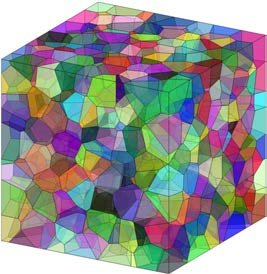
\includegraphics[scale=0.43]{Images/3D-Voronoi-tessellation-with-1000-grains-unit-cell-with-its-internal-grains-not.png}
%     \caption[3d Voronoi tessellation.]{An example of a Voronoi tesselation in 3d.}
%     \label{fig:3dvoronoi}
% \end{figure}

% In \citeauthor{colosimo_complex_2022} (2022), the authors aim to compare the nominal slices with the actual slices measured through x-ray computed tomography of a lattice structure composed of 64 dodecahedron unit cells of size \SI{10}{\milli\metre} within a specimen of $40 \times 40 \times 40$ \unit{\milli\metre}. Subsequntely, the 2D image of the as-built single cell and as-designed one were compared, slice by slice, in order to compute the deviation index. Given a pair of images that correspond to the $z-$th slice of the as-designed cell and the $z-$th slice of the as-built cell, let $i_{u,v,z}(\text{as.designed}$ and let $i_{u,v,z}(\text{as.build}$ be the intensities of $(u,v)^{th}$ pixel in the as-designed slice and in the as-built slice, respectively. In Fig. \ref{fig:slices} there are some examples of the procedure. A superimposition of these two images leads to four possible cases:
% \begin{itemize}
%     \item Region 1: pixels in which both $i_{u,v,z}(\text{as.designed})=0$ and $i_{u,v,z}(\text{as.build})=0$, i.e., pixels where material is present in both the images.
%     \item Region 2: pixels in which both $i_{u,v,z}(\text{as.designed})=1$ and $i_{u,v,z}(\text{as.build})=1$, i.e., pixels that correspond to the background in both the images.
%     \item Region 3: pixels in which both $i_{u,v,z}(\text{as.designed})=0$ and $i_{u,v,z}(\text{as.build})=1$, i.e., pixels where material is present in the as-designed slice but not in the as-built slice (i.e., less material has been produced than indicated in the CAD model)
%     \item Region 4: pixels in which both $i_{u,v,z}(\text{as.designed})=1$ and $i_{u,v,z}(\text{as.build})=0$, i.e. pixels where material is present in the as-built slice but not in the as-designed slice (i.e., more material has been produced than indicated in to the CAD model).
% \end{itemize}


% \begin{figure}
%     \centering
%     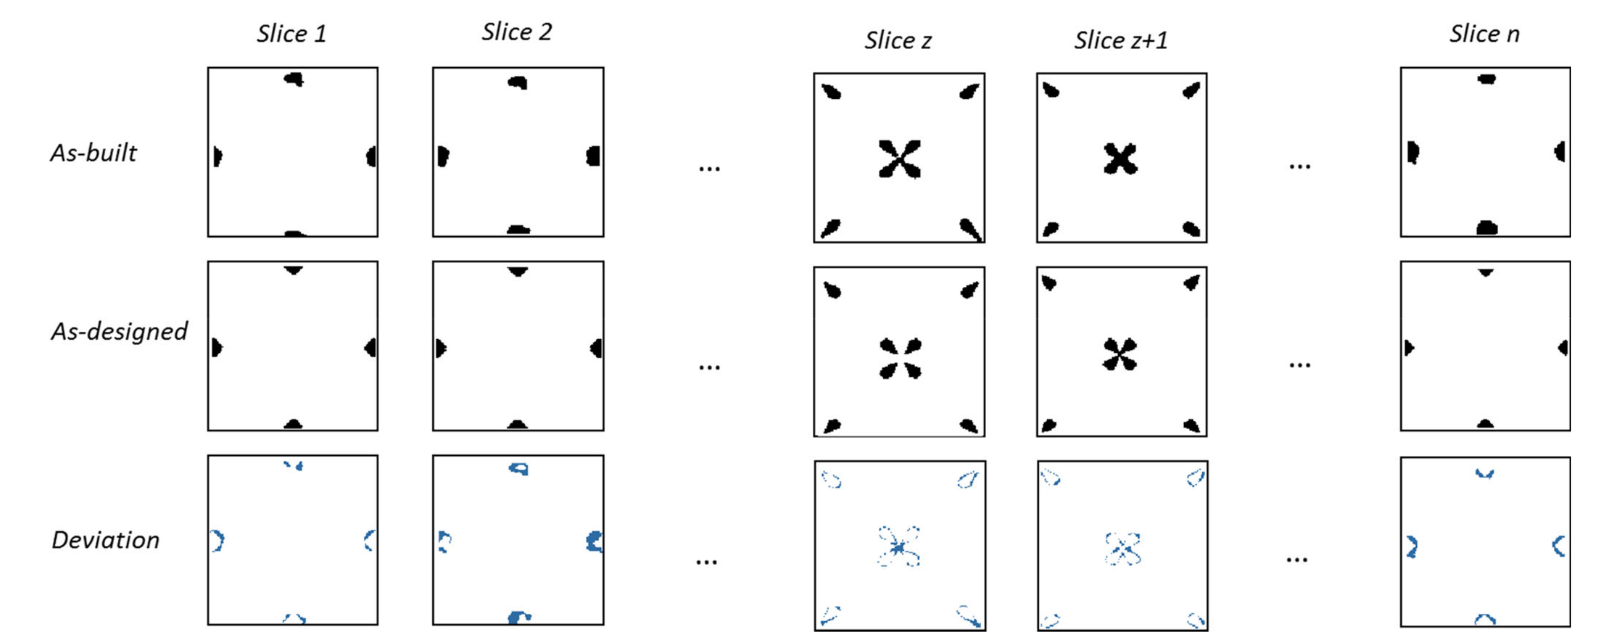
\includegraphics[scale=0.5]{Images/slicescolosimo.png}
%     \caption[Deviation index.]{Example of as-built (top row) and as-designed (central row) slice images at different z heights with the corresponding deviation (bottom row) \cite{colosimo_complex_2022}. }
%     \label{fig:slices}
% \end{figure}


% The overall number of pixels that belong to the union of region 3 or region 4 is the number of pixels for which $i_{u,v,z}(\text{as.build}) - i_{u,v,z}(\text{as.designed}) \neq 0$. So the \emph{deviation index} for the cell $(i,j,k)$ is defined as
% \begin{equation}
% \label{eq:deviationindex}
% \delta_{i, j, k}(z)= \sum_{u=1}^p \sum_{v=1}^p \mathcal{I}\left(i_{u, v, z}(\text { as.built })\right. -i_{u, v, z}(\text { as.designed })\neq 0)_{i, j, k},
% \end{equation}
% where $\mathcal{I}$ is the indicator function, that is 1 if the condition in brackets is true and 0 otherwise.
% After calculating the deviation index for each cell, the authors suggest using a cubic B-splines basis to fit a functional profile on the deviation index as a function of the slice position along cell z-axis. The position of the knots was chosen to eliminate the first and second discontinuity present in the deviation profiles, resulting from the typical trabecular structure of lattice designs. Fixed knots were then placed at the discontinuities of the as-designed geometry. Subsequently, intermediate knots were added iteratively, until a knee in the mean squared error (MSE) scree plot of the B-spline model residuals was identified.
% At the conclusion of step 5 in Fig. \ref{fig:colosimofunctional}, as outlined in the article, we will have 64 functional profiles, one for each cell. These profiles and the centroid of each cell in a lattice in $\mathbb{R}^3$ and will be the input for the classification algorithm described in Section \ref{sec:bvc}. In doing so, we could identify if there are critical areas within the lattice where cells exhibit similar anomalous behavior. Coupled with the ability to quantify the magnitude of the defect using the functional profiles, this could lead to a deeper understanding of the lattice structure's behavior and determine whether, despite its imperfections, it remains fit for its intended use. Indeed, localized geometric and dimensional deviations of the unit cells might adversely affect the structure's elastic modulus and compressive strength \cite{colosimo_complex_2022}.

% \begin{figure}
%     \centering
%     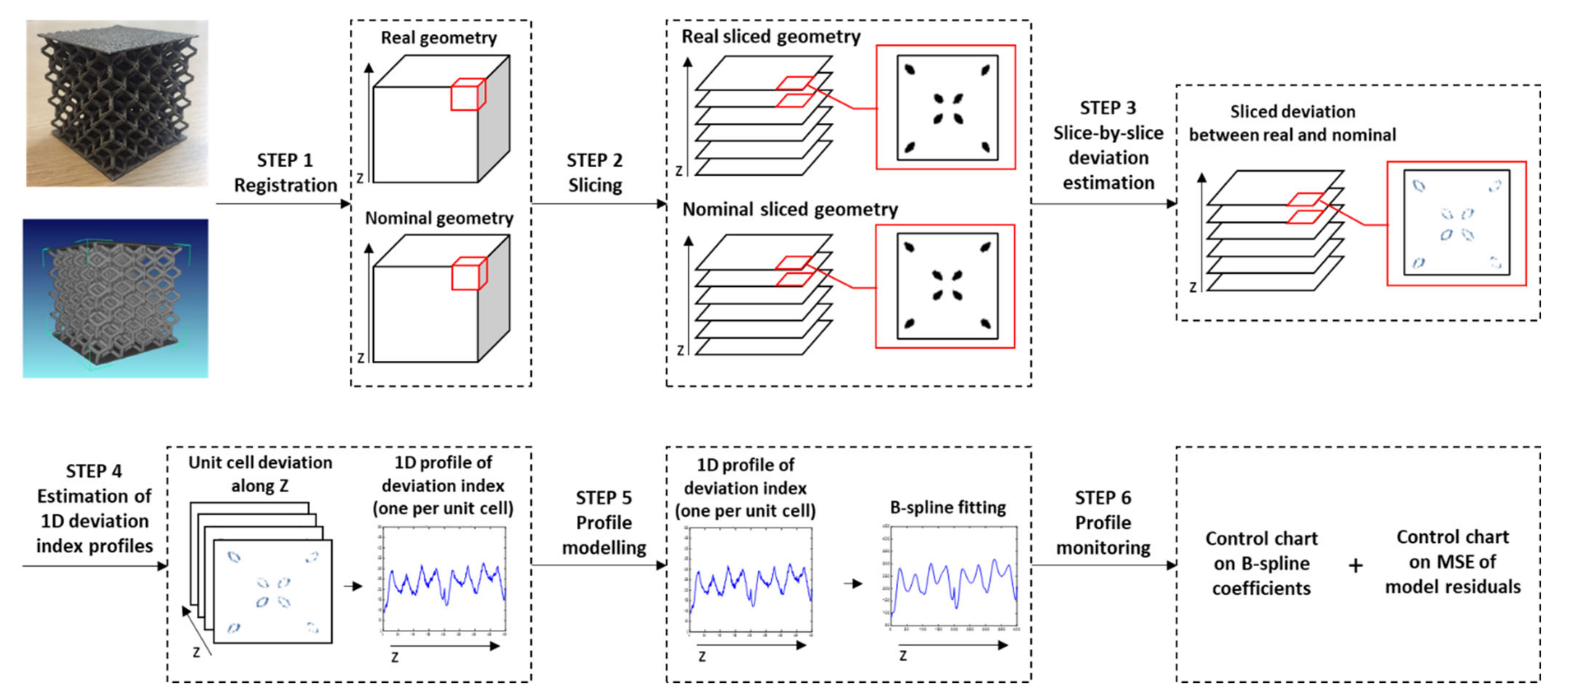
\includegraphics[scale=0.5]{Images/colosimosplines.png}
%     \caption[Functional control chart in complex geometries.]{Schema of the proposed methodology in \cite{colosimo_complex_2022}. The output of step 5 would be the input for the classification algorithm.}
%     \label{fig:colosimofunctional}
% \end{figure}
% % <<< End of Succesful case of the algorithm


%>>> Simulation Study
\section{Simulation Study}
\label{sec:simstudy}

% <<< End of Simulation Study

%As we will see in Section \ref{sec:bvc}, the number $K$ of clusters is an input of the algorithm, making hierarchical clustering not suitable for our purposes. But before delving into the algorithm's description, I also want to explain the concept of \textit{bagging} for clustering. It is based on the concept of bootstrapping. Bootstrapping is a resampling technique that helps in finding more reliable results from a clustering algorithm. In the algorithm, we will perform multiple clustering "rounds" in order to find a frequency distribution of the belongings of the observation to a specific cluster. The final cluster label for each observation will be the "most probable correct result" by majority voting.